% Options for packages loaded elsewhere
\PassOptionsToPackage{unicode}{hyperref}
\PassOptionsToPackage{hyphens}{url}
%
\documentclass[
]{article}
\usepackage{lmodern}
\usepackage{amssymb,amsmath}
\usepackage{ifxetex,ifluatex}
\ifnum 0\ifxetex 1\fi\ifluatex 1\fi=0 % if pdftex
  \usepackage[T1]{fontenc}
  \usepackage[utf8]{inputenc}
  \usepackage{textcomp} % provide euro and other symbols
\else % if luatex or xetex
  \usepackage{unicode-math}
  \defaultfontfeatures{Scale=MatchLowercase}
  \defaultfontfeatures[\rmfamily]{Ligatures=TeX,Scale=1}
\fi
% Use upquote if available, for straight quotes in verbatim environments
\IfFileExists{upquote.sty}{\usepackage{upquote}}{}
\IfFileExists{microtype.sty}{% use microtype if available
  \usepackage[]{microtype}
  \UseMicrotypeSet[protrusion]{basicmath} % disable protrusion for tt fonts
}{}
\makeatletter
\@ifundefined{KOMAClassName}{% if non-KOMA class
  \IfFileExists{parskip.sty}{%
    \usepackage{parskip}
  }{% else
    \setlength{\parindent}{0pt}
    \setlength{\parskip}{6pt plus 2pt minus 1pt}}
}{% if KOMA class
  \KOMAoptions{parskip=half}}
\makeatother
\usepackage{xcolor}
\IfFileExists{xurl.sty}{\usepackage{xurl}}{} % add URL line breaks if available
\IfFileExists{bookmark.sty}{\usepackage{bookmark}}{\usepackage{hyperref}}
\hypersetup{
  pdftitle={Introduction to statistics},
  pdfauthor={Alex Riley},
  hidelinks,
  pdfcreator={LaTeX via pandoc}}
\urlstyle{same} % disable monospaced font for URLs
\usepackage[margin=1in]{geometry}
\usepackage{color}
\usepackage{fancyvrb}
\newcommand{\VerbBar}{|}
\newcommand{\VERB}{\Verb[commandchars=\\\{\}]}
\DefineVerbatimEnvironment{Highlighting}{Verbatim}{commandchars=\\\{\}}
% Add ',fontsize=\small' for more characters per line
\usepackage{framed}
\definecolor{shadecolor}{RGB}{248,248,248}
\newenvironment{Shaded}{\begin{snugshade}}{\end{snugshade}}
\newcommand{\AlertTok}[1]{\textcolor[rgb]{0.94,0.16,0.16}{#1}}
\newcommand{\AnnotationTok}[1]{\textcolor[rgb]{0.56,0.35,0.01}{\textbf{\textit{#1}}}}
\newcommand{\AttributeTok}[1]{\textcolor[rgb]{0.77,0.63,0.00}{#1}}
\newcommand{\BaseNTok}[1]{\textcolor[rgb]{0.00,0.00,0.81}{#1}}
\newcommand{\BuiltInTok}[1]{#1}
\newcommand{\CharTok}[1]{\textcolor[rgb]{0.31,0.60,0.02}{#1}}
\newcommand{\CommentTok}[1]{\textcolor[rgb]{0.56,0.35,0.01}{\textit{#1}}}
\newcommand{\CommentVarTok}[1]{\textcolor[rgb]{0.56,0.35,0.01}{\textbf{\textit{#1}}}}
\newcommand{\ConstantTok}[1]{\textcolor[rgb]{0.00,0.00,0.00}{#1}}
\newcommand{\ControlFlowTok}[1]{\textcolor[rgb]{0.13,0.29,0.53}{\textbf{#1}}}
\newcommand{\DataTypeTok}[1]{\textcolor[rgb]{0.13,0.29,0.53}{#1}}
\newcommand{\DecValTok}[1]{\textcolor[rgb]{0.00,0.00,0.81}{#1}}
\newcommand{\DocumentationTok}[1]{\textcolor[rgb]{0.56,0.35,0.01}{\textbf{\textit{#1}}}}
\newcommand{\ErrorTok}[1]{\textcolor[rgb]{0.64,0.00,0.00}{\textbf{#1}}}
\newcommand{\ExtensionTok}[1]{#1}
\newcommand{\FloatTok}[1]{\textcolor[rgb]{0.00,0.00,0.81}{#1}}
\newcommand{\FunctionTok}[1]{\textcolor[rgb]{0.00,0.00,0.00}{#1}}
\newcommand{\ImportTok}[1]{#1}
\newcommand{\InformationTok}[1]{\textcolor[rgb]{0.56,0.35,0.01}{\textbf{\textit{#1}}}}
\newcommand{\KeywordTok}[1]{\textcolor[rgb]{0.13,0.29,0.53}{\textbf{#1}}}
\newcommand{\NormalTok}[1]{#1}
\newcommand{\OperatorTok}[1]{\textcolor[rgb]{0.81,0.36,0.00}{\textbf{#1}}}
\newcommand{\OtherTok}[1]{\textcolor[rgb]{0.56,0.35,0.01}{#1}}
\newcommand{\PreprocessorTok}[1]{\textcolor[rgb]{0.56,0.35,0.01}{\textit{#1}}}
\newcommand{\RegionMarkerTok}[1]{#1}
\newcommand{\SpecialCharTok}[1]{\textcolor[rgb]{0.00,0.00,0.00}{#1}}
\newcommand{\SpecialStringTok}[1]{\textcolor[rgb]{0.31,0.60,0.02}{#1}}
\newcommand{\StringTok}[1]{\textcolor[rgb]{0.31,0.60,0.02}{#1}}
\newcommand{\VariableTok}[1]{\textcolor[rgb]{0.00,0.00,0.00}{#1}}
\newcommand{\VerbatimStringTok}[1]{\textcolor[rgb]{0.31,0.60,0.02}{#1}}
\newcommand{\WarningTok}[1]{\textcolor[rgb]{0.56,0.35,0.01}{\textbf{\textit{#1}}}}
\usepackage{graphicx}
\makeatletter
\def\maxwidth{\ifdim\Gin@nat@width>\linewidth\linewidth\else\Gin@nat@width\fi}
\def\maxheight{\ifdim\Gin@nat@height>\textheight\textheight\else\Gin@nat@height\fi}
\makeatother
% Scale images if necessary, so that they will not overflow the page
% margins by default, and it is still possible to overwrite the defaults
% using explicit options in \includegraphics[width, height, ...]{}
\setkeys{Gin}{width=\maxwidth,height=\maxheight,keepaspectratio}
% Set default figure placement to htbp
\makeatletter
\def\fps@figure{htbp}
\makeatother
\setlength{\emergencystretch}{3em} % prevent overfull lines
\providecommand{\tightlist}{%
  \setlength{\itemsep}{0pt}\setlength{\parskip}{0pt}}
\setcounter{secnumdepth}{-\maxdimen} % remove section numbering

\title{Introduction to statistics}
\author{Alex Riley}
\date{8/25/2020}

\begin{document}
\maketitle

\hypertarget{introduction}{%
\section{Introduction}\label{introduction}}

Welcome to your first IB 372 lab!

In this lab we'll be going over introductory statistics, a topic that
will set you up for the data analysis and interpretation you'll be doing
throughout the semester and throughout your careers in just about any
field going forward.

We'll go over two major types of statistics, \textbf{descriptive}
statistics, and \textbf{inferential} statistics, as well as covering the
basics of how to read data into R, and explore that data with these
statistics.

By the end of this lab, you should be able to apply descriptive and
inferential statistics to a data set, define common statistical terms,
and be able to interperate the output of each analysis described here.

NOTE, THIS LAB GOES WITH THE LAB 1 R MARKDOWN (.Rmd) FILE! THAT IS WHERE
ALL QUESTIONS AND EXCERSISES REFFERED TO HERE WILL BE, MAKE SURE AFTER
EACH SECTION OF THIS DOCUMENT YOU GO TO THAT FILE AND WORK THROUGH THE
CORRESPONDING SECTION!

Also if you're looking at this in R studio directly, you should either
open the HTML version available, or click ``Knit'' on the row of tools
above this text to get it to the html format. You might have to install
a library or two for that, so I would recommend working from the pre
compiled version in html, but eventually you will likely turn things in
after ``knitting them'' into a more readable format, so feel free to get
that set up as well!

\hypertarget{getting-into-a-data-set}{%
\section{Getting into a data set}\label{getting-into-a-data-set}}

For today's lab, you'll be using several data sets that you'll read into
R from files we provide, but we'll start out demonstrating a few
concepts with a data set provided with every R installation, first off
let's use the data set called ``iris''.

Because this data set is included with R, we can import it by just using
the following code

\begin{Shaded}
\begin{Highlighting}[]
\CommentTok{\#read in the data set called iris}
\KeywordTok{data}\NormalTok{(}\StringTok{"iris"}\NormalTok{)}
\end{Highlighting}
\end{Shaded}

This dataset contains measurements on individuals of three different
iris species, and was first published by a famous biologist and
statistician names Ronald Fisher

Let's get a look at what we actually have data on shall we?

\begin{Shaded}
\begin{Highlighting}[]
\CommentTok{\#the dim function tells us the dimensions of our data set, how many rows and columns of data we have}
\KeywordTok{dim}\NormalTok{(iris)}
\end{Highlighting}
\end{Shaded}

\begin{verbatim}
## [1] 150   5
\end{verbatim}

\begin{Shaded}
\begin{Highlighting}[]
\CommentTok{\#we use the head function to see the top few rows of a data set}
\KeywordTok{head}\NormalTok{(iris)}
\end{Highlighting}
\end{Shaded}

\begin{verbatim}
##   Sepal.Length Sepal.Width Petal.Length Petal.Width Species
## 1          5.1         3.5          1.4         0.2  setosa
## 2          4.9         3.0          1.4         0.2  setosa
## 3          4.7         3.2          1.3         0.2  setosa
## 4          4.6         3.1          1.5         0.2  setosa
## 5          5.0         3.6          1.4         0.2  setosa
## 6          5.4         3.9          1.7         0.4  setosa
\end{verbatim}

We can get a lot of useful information about our data from just these
two functions in R (a function in R is just like a function in your old
math class, it's anything that takes one thing in, does something with
it, and spits something else out).

From the output of running dim on our data set, we can see that we have
150 rows of our data set, which correspond to 150 iris
\textbf{individuals}, and 5 columns of our data, which correspond to 5
\textbf{variables}, or things that were measured

This is where I type something super obvious that's important to keep in
mind.

If we take the entire global population of each of these species and
count them, there would be more than 150 individuals, because we're
grouping based on species, we would call the group of all individuals of
a given species of iris the \textbf{population} of that species. A
population is just the total number of plants/animals/people that have
an attribute of interest. A \textbf{parameter} is the real measure of
this attribute for the population. We say there are \textbf{N}
individuals when we're talking about a whole population.

Alternatively, our data set is a \textbf{sample} of each of those
populations, a subset of the population for which a researcher measures
the attribute. This sample is assumed to be representative of the entire
population. A \textbf{statistic} is a measure of the attribute for the
sample. When we're talking about a sample we say there are \textbf{n}
individuals.

So for our data set, n=150, it is a sample of the global iris
population.

From the output of running head on our data set, we can see that the 5
variables included here are Sepal length, Sepal width, Petal length,
Petal width, and species, if you're wondering why there are dots in the
names of each variable, it's because including spaces in column names
makes it harder to work with in R, keep that in mind as you collect your
own data!

We can also see from our head function that we've got two different
types of variables here, the first four columns are measurements of
length or width. These are called \textbf{continuous} variables, they
can be any value in an uninterrupted range (if you picture a number
line, they can be any value on there). Species on the other hand is not
a continuous variable, let's see if there are any values other than
setosa, which is all we see in the first few lines.

\begin{Shaded}
\begin{Highlighting}[]
\CommentTok{\#we use unique to get all the unique values in a set a of data}
\CommentTok{\#the $ after iris tells R we want a column within that data set, in this case, species}
\KeywordTok{unique}\NormalTok{(iris}\OperatorTok{$}\NormalTok{Species)}
\end{Highlighting}
\end{Shaded}

\begin{verbatim}
## [1] setosa     versicolor virginica 
## Levels: setosa versicolor virginica
\end{verbatim}

We see here that we've got three ``levels'' of this variable, but they
aren't numbers like our other variables. This is what's called a
\textbf{nominal discrete} variable, which just means a variable where
only certain values are possible (the species of iris), and the options,
or levels, don't have a meaningful order. If there were a meaningful
order to our possible values, we would have an \textbf{ordered discrete}
variable, which could be something like shoe size, it's a number, and
each size fits into an order, however there are a limited number of
possible values.

\hypertarget{descriptive-statistics}{%
\section{Descriptive statistics}\label{descriptive-statistics}}

Now that we have a data set, and understand what we're looking at, let's
start to get an idea of what our data look like quantitatively. When
we're not looking to rigorously answer a specific, quantitative
question, like ``are the sepals of species A longer than the sepals of
species B'', then use what we call \textbf{descriptive} statistics,
these are values like \textbf{mean}, \textbf{median}, and \textbf{mode},
that just give us a way to quantitatively describe our data.

The best way to get started looking at a data set, is with just a simple
histogram and R makes this really easy for us. Here we're going to make
a histogram of our sepal width

\begin{Shaded}
\begin{Highlighting}[]
\CommentTok{\#the hist function allows us to draw a histogram of a data set}
\KeywordTok{hist}\NormalTok{(iris}\OperatorTok{$}\NormalTok{Sepal.Width)}
\end{Highlighting}
\end{Shaded}

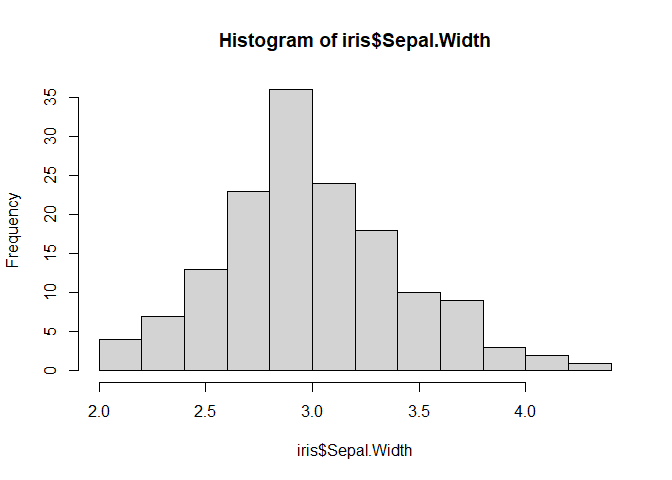
\includegraphics{Introduction_to_stats_files/figure-latex/histogram-1.pdf}

This is useful because it allows us to get a look at how our data is
distributed across the range of values represented, and give us a
qualitative idea of what we're looking at.

As a brief, but important tangent, it's always important to keep in mind
how you're visualizing your data, as well as what data your visualizing.
With histograms the biggest factor to consider is, how are we breaking
up our data, or how wide a range of values are we grouping together.
This is important because if don't have enough groups we may clump too
many individual together and it can be hard to notice a pattern.

\begin{Shaded}
\begin{Highlighting}[]
\CommentTok{\#we can use the breaks argument in hist to tell it how many breaks we want in our histogram}
\KeywordTok{hist}\NormalTok{(iris}\OperatorTok{$}\NormalTok{Sepal.Width, }\DataTypeTok{breaks =} \DecValTok{3}\NormalTok{)}
\end{Highlighting}
\end{Shaded}

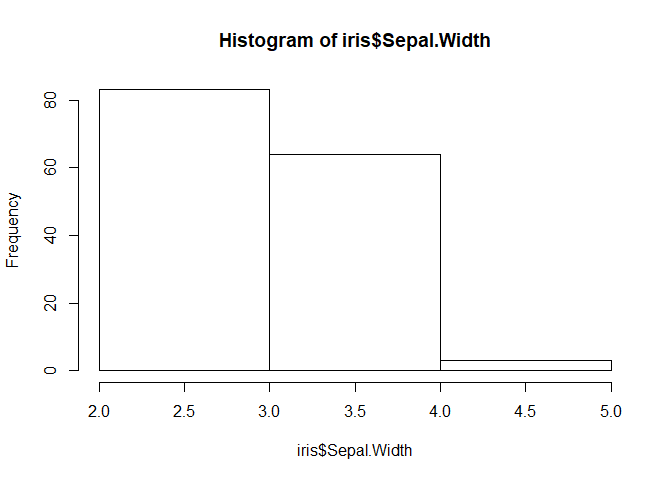
\includegraphics{Introduction_to_stats_files/figure-latex/notEnoughBreaks-1.pdf}

Here we don't break up our data enough and we miss out on the major
structure of our data (that it's approximately normally distributed, but
we'll get to that soon!). Alternatively, if we break up our data too
much, we can notice patterns that aren't particularly meaningful (this
is a judgement call that you'll get better at as you spend more time
with real data sets!).

\begin{Shaded}
\begin{Highlighting}[]
\KeywordTok{hist}\NormalTok{(iris}\OperatorTok{$}\NormalTok{Sepal.Width, }\DataTypeTok{breaks =} \DecValTok{45}\NormalTok{)}
\end{Highlighting}
\end{Shaded}

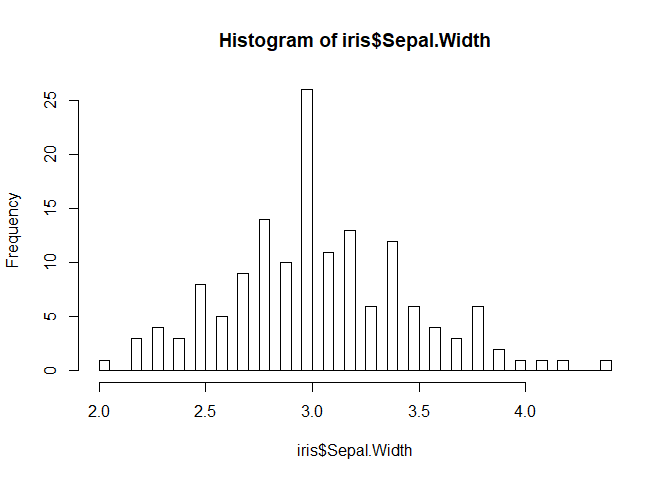
\includegraphics{Introduction_to_stats_files/figure-latex/tooManyBreaks-1.pdf}

Now we can see the same main pattern as we did in our original
histogram, however we also see a lot more rises and drops from column to
column. It doesn't take away much from the main pattern in this case,
but it can throw us off of a meaningful signal in our data when we have
messier data sets. How many breaks you include in a histogram is your
choice, but always try out a few different ways to break up your data to
make sure you're getting a real signal and not missing anything!

Now lets learn what values we can find for our data to start to
understand what we're looking at!

\hypertarget{measures-of-central-tendency}{%
\subsection{Measures of central
tendency}\label{measures-of-central-tendency}}

The first set of descriptive statistics we'll look at here are what are
called \textbf{measures of central tendency}, which for our purposes is
really a fancy term for all the things your third grade math teacher
called averages, we'll look at \textbf{mean}, \textbf{median}, and
\textbf{mode}.

The most important of these values is the \textbf{mean}, which for a
\textbf{population} is called \(\mu\), and for a \textbf{sample} is
called \(\bar{x}\), you're all probably familiar with the formula for
mean, but as a refresher it's defined as the following for a sample:\\
\[ \bar{x} = \frac{\sum_{i=1}^n x_i}{n} \] Or, in English, just the sum
of all the values divided by the number of values.

The \textbf{median} is just the middle value in a set of data, if you're
data is in order and you have an odd number of values, the median is
just the value in the middle, or the \(\frac{n+1}{2}th\) value, so
\[ M_{odd} = x_\frac{n+1}{2}\]\\
If you've got an even number of values, because you may not have one
value in the middle, you take the average of the two numbers closest to
the middle, so \[M_{even} = \frac{x_\frac{n}{2}+x_\frac{n+1}{2}}{2}\]

The \textbf{mode}, on the other hand, is the most common value in a data
set.

For example, if we've got a data set of the values:
\[1,1,1,1,4,5,6,6,7,7,7,8,9,10\] then the \textbf{mean} = 5.214286 the
\textbf{median} = 6 and the \textbf{mode} = 1

If our data are \textbf{normally} distributed, think a symmetrical bell
curve, the mean is just at the peak of a histogram of the data, to
demonstrate that, here's a plot of some randomly simulated normal data,
with a red line representing the mean.

\begin{Shaded}
\begin{Highlighting}[]
\CommentTok{\#first we generate a random dataset of 100000 values from a noramal distribution}
\CommentTok{\#note that the \textless{}{-} assigns a value to a variable}
\NormalTok{x \textless{}{-}}\StringTok{ }\KeywordTok{rnorm}\NormalTok{(}\DecValTok{100000}\NormalTok{)}

\CommentTok{\#then we take it\textquotesingle{}s mean}
\NormalTok{xBar \textless{}{-}}\StringTok{ }\KeywordTok{mean}\NormalTok{(x)}

\CommentTok{\#we draw a histogram of the data}
\KeywordTok{hist}\NormalTok{(x, }\DataTypeTok{main =} \StringTok{"Normal data with mean"}\NormalTok{)}

\CommentTok{\#and add a line to the plot where the mean is}
\KeywordTok{abline}\NormalTok{(}\DataTypeTok{v=}\NormalTok{xBar, }\DataTypeTok{col=}\StringTok{"red"}\NormalTok{, }\DataTypeTok{lwd=}\DecValTok{2}\NormalTok{)}
\end{Highlighting}
\end{Shaded}

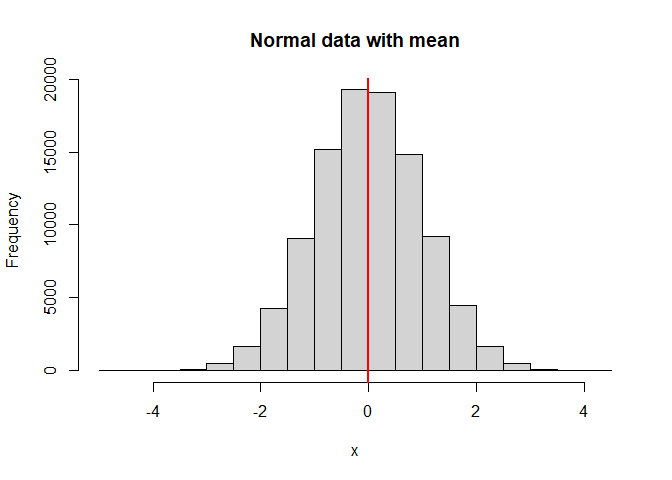
\includegraphics{Introduction_to_stats_files/figure-latex/normalData-1.pdf}

Interestingly, if the data is normal then the mode and median are also
right in the middle where the highest frequency is, it takes a little
bit of code that I'd rather not complicate things with for this example
to get the mode of our data in R, so I'm going to leave out a plot with
the mode, but here's one with the median in blue

\begin{Shaded}
\begin{Highlighting}[]
\CommentTok{\#get the median of the data and assign it to xMed}
\NormalTok{xMed \textless{}{-}}\StringTok{ }\KeywordTok{median}\NormalTok{(x)}

\CommentTok{\#we draw a histogram of the data}
\KeywordTok{hist}\NormalTok{(x, }\DataTypeTok{main =} \StringTok{"Normal data with Median"}\NormalTok{)}

\CommentTok{\#and add a line to the plot where the median is}
\KeywordTok{abline}\NormalTok{(}\DataTypeTok{v=}\NormalTok{xMed, }\DataTypeTok{col=}\StringTok{"blue"}\NormalTok{, }\DataTypeTok{lwd=}\DecValTok{2}\NormalTok{)}
\end{Highlighting}
\end{Shaded}

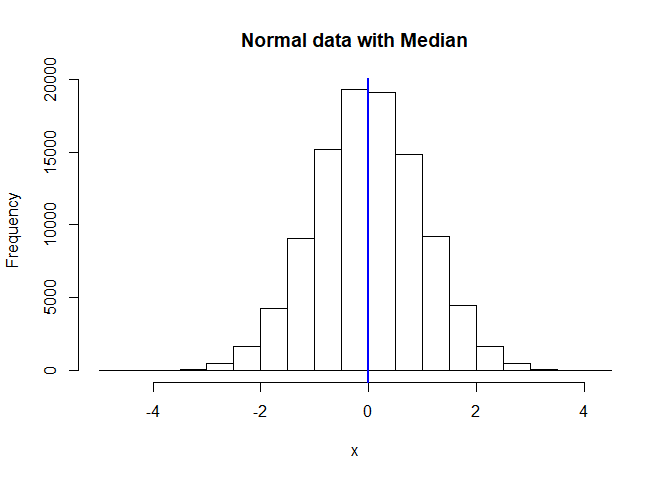
\includegraphics{Introduction_to_stats_files/figure-latex/modeAndMedian-1.pdf}

While measures of central tendency don't tell us much about how our data
are actually distributed, they can tell us if our data is
\textbf{skewed}, basically just whether or not our data are perfectly
symmetrical. If our \textbf{mean, median, and mode are all equal}, then
we know our data are symmetrical and \textbf{not skewed} in the negative
or positive direction, if our \textbf{mean is lower than our median and
mode} then we call our data \textbf{negatively skewed}, and if our
\textbf{mean is higher than our median and mode}, we say our data is
\textbf{positively skewed}, don't worry too much about knowing the
specifics of each of these terms, just know that not all data are
symmetrical, and if they aren't we say they're skewed.

That's all the measures of central tendency you need to know for most
applications, so now let's move on to measures of dispersion

\hypertarget{measures-of-dispersion}{%
\subsection{Measures of dispersion}\label{measures-of-dispersion}}

While we can tell a lot from the mean, median, and mode of a data set,
it's important to remember that they don't tell us everything about how
our data is distributed across its \textbf{range} - \(x_{max}-x_{min}\),
for example, these three plots all have the same exact mean, median, and
mode, but if you got these three data sets, you'd know something was
different between them

\begin{Shaded}
\begin{Highlighting}[]
\CommentTok{\#these are functions we use to randomly sample, and plot random normal data, don\textquotesingle{}t worry about these functions for now, unless you want to! in which case, feel free to worry about them!}
\CommentTok{\#least dispersion}
\NormalTok{x \textless{}{-}}\StringTok{ }\KeywordTok{seq}\NormalTok{(}\OperatorTok{{-}}\DecValTok{10}\NormalTok{, }\DecValTok{10}\NormalTok{, }\DataTypeTok{length=}\DecValTok{1000}\NormalTok{)}
\NormalTok{y \textless{}{-}}\StringTok{ }\KeywordTok{dnorm}\NormalTok{(x, }\DataTypeTok{mean=}\DecValTok{0}\NormalTok{, }\DataTypeTok{sd=}\NormalTok{.}\DecValTok{75}\NormalTok{)}
\KeywordTok{plot}\NormalTok{(x, y, }\DataTypeTok{type=}\StringTok{"l"}\NormalTok{, }\DataTypeTok{lwd=}\DecValTok{1}\NormalTok{)}
\end{Highlighting}
\end{Shaded}

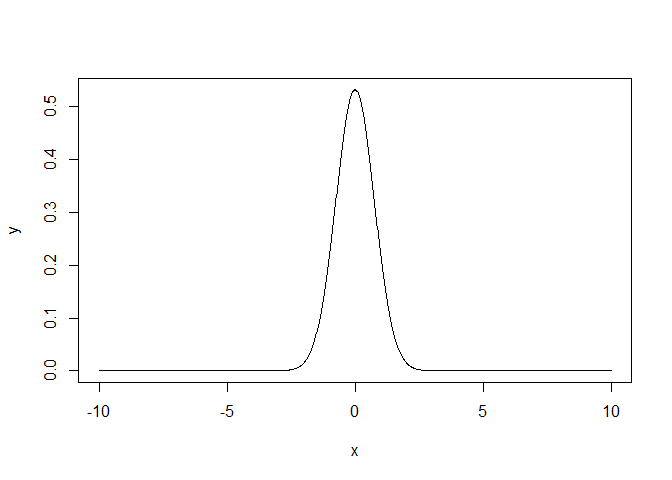
\includegraphics{Introduction_to_stats_files/figure-latex/whyWeCareAboutDispersion-1.pdf}

\begin{Shaded}
\begin{Highlighting}[]
\CommentTok{\#medium dispersion}
\NormalTok{x \textless{}{-}}\StringTok{ }\KeywordTok{seq}\NormalTok{(}\OperatorTok{{-}}\DecValTok{10}\NormalTok{, }\DecValTok{10}\NormalTok{, }\DataTypeTok{length=}\DecValTok{1000}\NormalTok{)}
\NormalTok{y \textless{}{-}}\StringTok{ }\KeywordTok{dnorm}\NormalTok{(x, }\DataTypeTok{mean=}\DecValTok{0}\NormalTok{, }\DataTypeTok{sd=}\DecValTok{2}\NormalTok{)}
\KeywordTok{plot}\NormalTok{(x, y, }\DataTypeTok{type=}\StringTok{"l"}\NormalTok{, }\DataTypeTok{lwd=}\DecValTok{1}\NormalTok{)}
\end{Highlighting}
\end{Shaded}

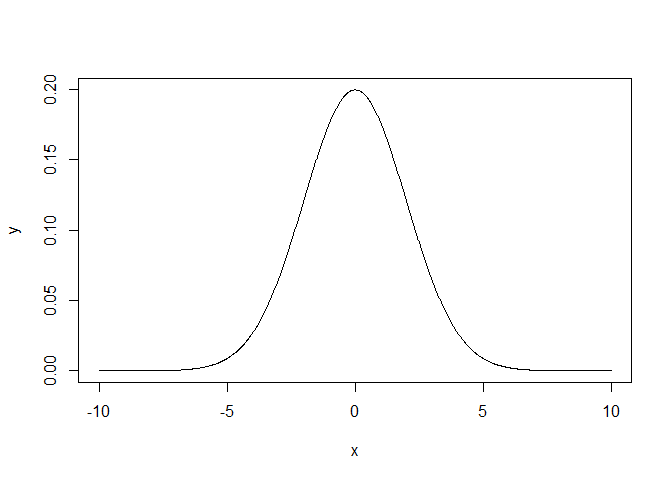
\includegraphics{Introduction_to_stats_files/figure-latex/whyWeCareAboutDispersion-2.pdf}

\begin{Shaded}
\begin{Highlighting}[]
\CommentTok{\#most dispersion}
\NormalTok{x \textless{}{-}}\StringTok{ }\KeywordTok{seq}\NormalTok{(}\OperatorTok{{-}}\DecValTok{10}\NormalTok{, }\DecValTok{10}\NormalTok{, }\DataTypeTok{length=}\DecValTok{1000}\NormalTok{)}
\NormalTok{y \textless{}{-}}\StringTok{ }\KeywordTok{dnorm}\NormalTok{(x, }\DataTypeTok{mean=}\DecValTok{0}\NormalTok{, }\DataTypeTok{sd=}\DecValTok{3}\NormalTok{)}
\KeywordTok{plot}\NormalTok{(x, y, }\DataTypeTok{type=}\StringTok{"l"}\NormalTok{, }\DataTypeTok{lwd=}\DecValTok{1}\NormalTok{)}
\end{Highlighting}
\end{Shaded}

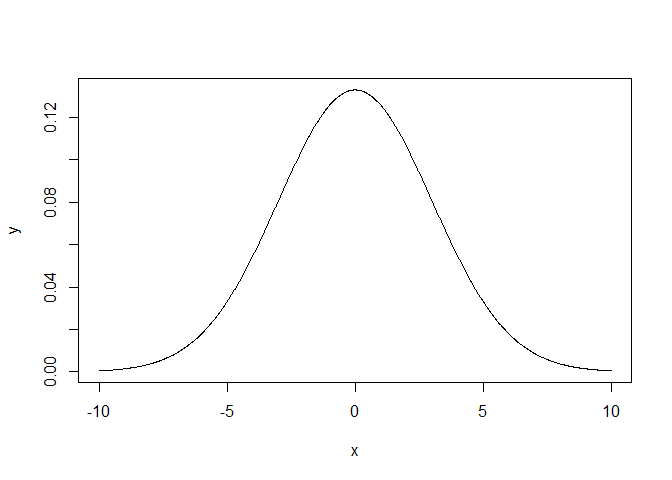
\includegraphics{Introduction_to_stats_files/figure-latex/whyWeCareAboutDispersion-3.pdf}
You'd be right in thinking they are different because they all have
different \textbf{standard deviations}

\textbf{Standard deviation}, generally represented as \(\sigma\) for a
population or \(s\) for a sample, is a measure of how spread out our
data is, it's really useful for understanding the normal distribution,
which I'll talk about in just a second.

While \textbf{standard deviation} is great, and has a straight forward
interpretation, we rarely calculate it directly, it's actually easier to
calculate the squared \textbf{standard deviation}, which we call
\textbf{variance} (\(\sigma^2\) for a population, or \(s^2\) for a
sample). The formula for variance is
\[s^2=\frac{\sum_{i=1}^{n}(x_i-\bar{x})^2}{n-1}\]\\
but we won't hold you responsible for having this memorized

The reason \textbf{standard deviation} is so useful is it allows us to
translate knowing that our data is normal, into knowing what proportion
of our data is where, for example in a perfect, normal data set, we know
that 68.2\% of our data falls within one standard deviation of the mean,
a 95\% chance it falls within 2 standard deviations ,and there's only a
0.2\% chance of getting a value more than 3 standard deviations from the
mean. Here are the same plots as above but with lines drawn in blue at
one standard deviation out, in red at two standard deviations out, and
in green at three standard deviations out.

\begin{Shaded}
\begin{Highlighting}[]
\CommentTok{\#least dispersion}
\NormalTok{x \textless{}{-}}\StringTok{ }\KeywordTok{seq}\NormalTok{(}\OperatorTok{{-}}\DecValTok{10}\NormalTok{, }\DecValTok{10}\NormalTok{, }\DataTypeTok{length=}\DecValTok{1000}\NormalTok{)}
\NormalTok{y \textless{}{-}}\StringTok{ }\KeywordTok{dnorm}\NormalTok{(x, }\DataTypeTok{mean=}\DecValTok{0}\NormalTok{, }\DataTypeTok{sd=}\NormalTok{.}\DecValTok{75}\NormalTok{)}
\NormalTok{y.stDev \textless{}{-}}\StringTok{ }\FloatTok{.75}
\KeywordTok{plot}\NormalTok{(x, y, }\DataTypeTok{type=}\StringTok{"l"}\NormalTok{, }\DataTypeTok{lwd=}\DecValTok{1}\NormalTok{)}
\KeywordTok{abline}\NormalTok{(}\DataTypeTok{v=}\NormalTok{y.stDev, }\DataTypeTok{col=}\StringTok{"blue"}\NormalTok{, }\DataTypeTok{lwd=}\DecValTok{2}\NormalTok{)}
\KeywordTok{abline}\NormalTok{(}\DataTypeTok{v=}\OperatorTok{{-}}\NormalTok{y.stDev, }\DataTypeTok{col=}\StringTok{"blue"}\NormalTok{, }\DataTypeTok{lwd=}\DecValTok{2}\NormalTok{)}
\KeywordTok{abline}\NormalTok{(}\DataTypeTok{v=}\DecValTok{2}\OperatorTok{*}\NormalTok{y.stDev, }\DataTypeTok{col=}\StringTok{"red"}\NormalTok{, }\DataTypeTok{lwd=}\DecValTok{2}\NormalTok{)}
\KeywordTok{abline}\NormalTok{(}\DataTypeTok{v=}\OperatorTok{{-}}\DecValTok{2}\OperatorTok{*}\NormalTok{y.stDev, }\DataTypeTok{col=}\StringTok{"red"}\NormalTok{, }\DataTypeTok{lwd=}\DecValTok{2}\NormalTok{)}
\KeywordTok{abline}\NormalTok{(}\DataTypeTok{v=}\DecValTok{3}\OperatorTok{*}\NormalTok{y.stDev, }\DataTypeTok{col=}\StringTok{"green"}\NormalTok{, }\DataTypeTok{lwd=}\DecValTok{2}\NormalTok{)}
\KeywordTok{abline}\NormalTok{(}\DataTypeTok{v=}\OperatorTok{{-}}\DecValTok{3}\OperatorTok{*}\NormalTok{y.stDev, }\DataTypeTok{col=}\StringTok{"green"}\NormalTok{, }\DataTypeTok{lwd=}\DecValTok{2}\NormalTok{)}
\end{Highlighting}
\end{Shaded}

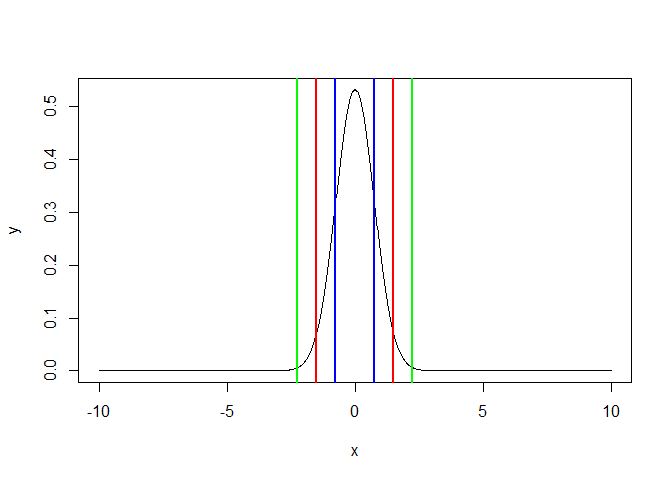
\includegraphics{Introduction_to_stats_files/figure-latex/sdDemoPlots-1.pdf}

\begin{Shaded}
\begin{Highlighting}[]
\CommentTok{\#medium dispersion}
\NormalTok{x \textless{}{-}}\StringTok{ }\KeywordTok{seq}\NormalTok{(}\OperatorTok{{-}}\DecValTok{10}\NormalTok{, }\DecValTok{10}\NormalTok{, }\DataTypeTok{length=}\DecValTok{1000}\NormalTok{)}
\NormalTok{y \textless{}{-}}\StringTok{ }\KeywordTok{dnorm}\NormalTok{(x, }\DataTypeTok{mean=}\DecValTok{0}\NormalTok{, }\DataTypeTok{sd=}\DecValTok{2}\NormalTok{)}
\NormalTok{y.stDev \textless{}{-}}\StringTok{ }\DecValTok{2}
\KeywordTok{plot}\NormalTok{(x, y, }\DataTypeTok{type=}\StringTok{"l"}\NormalTok{, }\DataTypeTok{lwd=}\DecValTok{1}\NormalTok{)}
\KeywordTok{abline}\NormalTok{(}\DataTypeTok{v=}\NormalTok{y.stDev, }\DataTypeTok{col=}\StringTok{"blue"}\NormalTok{, }\DataTypeTok{lwd=}\DecValTok{2}\NormalTok{)}
\KeywordTok{abline}\NormalTok{(}\DataTypeTok{v=}\OperatorTok{{-}}\NormalTok{y.stDev, }\DataTypeTok{col=}\StringTok{"blue"}\NormalTok{, }\DataTypeTok{lwd=}\DecValTok{2}\NormalTok{)}
\KeywordTok{abline}\NormalTok{(}\DataTypeTok{v=}\DecValTok{2}\OperatorTok{*}\NormalTok{y.stDev, }\DataTypeTok{col=}\StringTok{"red"}\NormalTok{, }\DataTypeTok{lwd=}\DecValTok{2}\NormalTok{)}
\KeywordTok{abline}\NormalTok{(}\DataTypeTok{v=}\OperatorTok{{-}}\DecValTok{2}\OperatorTok{*}\NormalTok{y.stDev, }\DataTypeTok{col=}\StringTok{"red"}\NormalTok{, }\DataTypeTok{lwd=}\DecValTok{2}\NormalTok{)}
\KeywordTok{abline}\NormalTok{(}\DataTypeTok{v=}\DecValTok{3}\OperatorTok{*}\NormalTok{y.stDev, }\DataTypeTok{col=}\StringTok{"green"}\NormalTok{, }\DataTypeTok{lwd=}\DecValTok{2}\NormalTok{)}
\KeywordTok{abline}\NormalTok{(}\DataTypeTok{v=}\OperatorTok{{-}}\DecValTok{3}\OperatorTok{*}\NormalTok{y.stDev, }\DataTypeTok{col=}\StringTok{"green"}\NormalTok{, }\DataTypeTok{lwd=}\DecValTok{2}\NormalTok{)}
\end{Highlighting}
\end{Shaded}

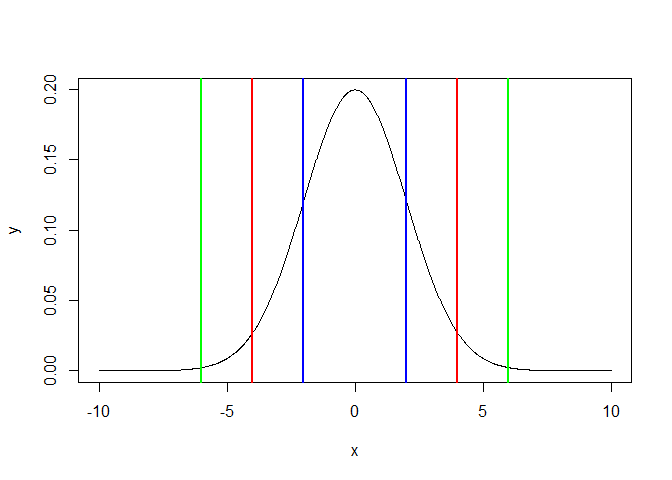
\includegraphics{Introduction_to_stats_files/figure-latex/sdDemoPlots-2.pdf}

\begin{Shaded}
\begin{Highlighting}[]
\CommentTok{\#most dispersion}
\NormalTok{x \textless{}{-}}\StringTok{ }\KeywordTok{seq}\NormalTok{(}\OperatorTok{{-}}\DecValTok{10}\NormalTok{, }\DecValTok{10}\NormalTok{, }\DataTypeTok{length=}\DecValTok{1000}\NormalTok{)}
\NormalTok{y \textless{}{-}}\StringTok{ }\KeywordTok{dnorm}\NormalTok{(x, }\DataTypeTok{mean=}\DecValTok{0}\NormalTok{, }\DataTypeTok{sd=}\DecValTok{3}\NormalTok{)}
\NormalTok{y.stDev \textless{}{-}}\StringTok{ }\DecValTok{3}
\KeywordTok{plot}\NormalTok{(x, y, }\DataTypeTok{type=}\StringTok{"l"}\NormalTok{, }\DataTypeTok{lwd=}\DecValTok{1}\NormalTok{)}
\KeywordTok{abline}\NormalTok{(}\DataTypeTok{v=}\NormalTok{y.stDev, }\DataTypeTok{col=}\StringTok{"blue"}\NormalTok{, }\DataTypeTok{lwd=}\DecValTok{2}\NormalTok{)}
\KeywordTok{abline}\NormalTok{(}\DataTypeTok{v=}\OperatorTok{{-}}\NormalTok{y.stDev, }\DataTypeTok{col=}\StringTok{"blue"}\NormalTok{, }\DataTypeTok{lwd=}\DecValTok{2}\NormalTok{)}
\KeywordTok{abline}\NormalTok{(}\DataTypeTok{v=}\DecValTok{2}\OperatorTok{*}\NormalTok{y.stDev, }\DataTypeTok{col=}\StringTok{"red"}\NormalTok{, }\DataTypeTok{lwd=}\DecValTok{2}\NormalTok{)}
\KeywordTok{abline}\NormalTok{(}\DataTypeTok{v=}\OperatorTok{{-}}\DecValTok{2}\OperatorTok{*}\NormalTok{y.stDev, }\DataTypeTok{col=}\StringTok{"red"}\NormalTok{, }\DataTypeTok{lwd=}\DecValTok{2}\NormalTok{)}
\KeywordTok{abline}\NormalTok{(}\DataTypeTok{v=}\DecValTok{3}\OperatorTok{*}\NormalTok{y.stDev, }\DataTypeTok{col=}\StringTok{"green"}\NormalTok{, }\DataTypeTok{lwd=}\DecValTok{2}\NormalTok{)}
\KeywordTok{abline}\NormalTok{(}\DataTypeTok{v=}\OperatorTok{{-}}\DecValTok{3}\OperatorTok{*}\NormalTok{y.stDev, }\DataTypeTok{col=}\StringTok{"green"}\NormalTok{, }\DataTypeTok{lwd=}\DecValTok{2}\NormalTok{)}
\end{Highlighting}
\end{Shaded}

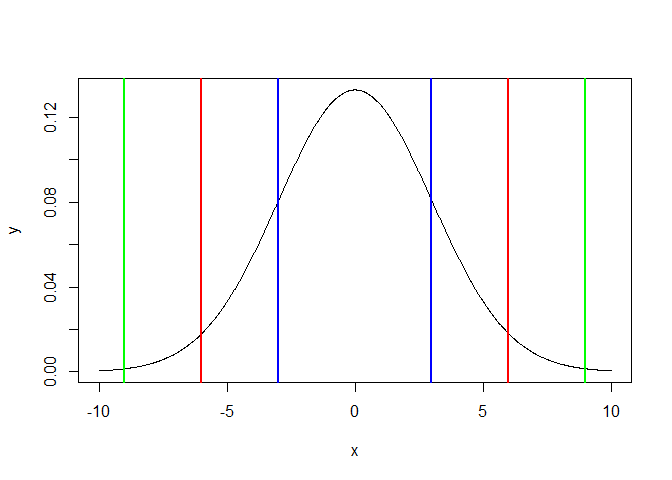
\includegraphics{Introduction_to_stats_files/figure-latex/sdDemoPlots-3.pdf}

In addition to \textbf{range}, \textbf{standard deviation}, and
\textbf{variance}, it's also helpful to have an understanding of
\textbf{standard error}, while we won't spend much time on it here,
standard error gives us a value to compare how well a sample mean
estimates the population mean, it's value is \[\frac{s}{\sqrt{n}}\]\\
so the larger our sample (n) the smaller our error is, and the higher
our standard deviation (s), the larger it is

\hypertarget{now-with-iris-data}{%
\subsection{Now with iris data!}\label{now-with-iris-data}}

Let's take what we've learned about descriptive statistics, and apply
them to our sepal length data for our iris species!

First, let's get measures of central tendency. We'll forego mode here
because we can get all the information we need here from our mean and
median, and R can calculate them with build in functions

\begin{Shaded}
\begin{Highlighting}[]
\CommentTok{\#mean}
\KeywordTok{mean}\NormalTok{(iris}\OperatorTok{$}\NormalTok{Sepal.Width)}
\end{Highlighting}
\end{Shaded}

\begin{verbatim}
## [1] 3.057333
\end{verbatim}

\begin{Shaded}
\begin{Highlighting}[]
\CommentTok{\#median}
\KeywordTok{median}\NormalTok{(iris}\OperatorTok{$}\NormalTok{Sepal.Width)}
\end{Highlighting}
\end{Shaded}

\begin{verbatim}
## [1] 3
\end{verbatim}

You might be thinking, OH MY GOSH! OUR MEAN AND MEDIAN AREN'T EQUAL SO
OUR DATA ISN'T NORMAL!!!!, HOW CAN WE USE ANY OF WHAT WE LEARN TODAY
(spoiler alert, lots of what we learn today requires normal data) IF OUR
DATA ISN'T NORMAL???, and you'd technically be right, having a mean and
median that are different does mean our data is skewed, but the
difference is so small it's effectively meaningless here, even with data
much more skewed than this people often assume normality, or if they
can't will apply a function to their data to make it more normal,
because a huge amount of the work done in statistics is on how to tell
things about normal, or normalized data sets.

We won't spend much time on them, but you should also be aware that
there are statistical tests and inferences we can make based on data
that isn't normalized (called non-parametric statistics), or based on
data that fit other distributions (Poisson, chi-squared, etc.). We'll
focus on normal, or almost normal data here, because it makes the
statistical tests we run much more straightforward!

Now that we know our data is approximately normal (we won't actually run
a formal test of this, we're basing it on the histogram and the
approximately equal mean and median), we can move on to characterize the
dispersion of our data.

\begin{Shaded}
\begin{Highlighting}[]
\CommentTok{\#range (min then max)}
\KeywordTok{range}\NormalTok{(iris}\OperatorTok{$}\NormalTok{Sepal.Width)}
\end{Highlighting}
\end{Shaded}

\begin{verbatim}
## [1] 2.0 4.4
\end{verbatim}

\begin{Shaded}
\begin{Highlighting}[]
\CommentTok{\#variance}
\KeywordTok{var}\NormalTok{(iris}\OperatorTok{$}\NormalTok{Sepal.Width)}
\end{Highlighting}
\end{Shaded}

\begin{verbatim}
## [1] 0.1899794
\end{verbatim}

\begin{Shaded}
\begin{Highlighting}[]
\CommentTok{\#standard deviation}
\CommentTok{\#sd gives us standard deviation, but we assign it to a variable here so we can calculate standard error}
\NormalTok{standardDev \textless{}{-}}\StringTok{ }\KeywordTok{sd}\NormalTok{(iris}\OperatorTok{$}\NormalTok{Sepal.Width)}
\NormalTok{standardDev}
\end{Highlighting}
\end{Shaded}

\begin{verbatim}
## [1] 0.4358663
\end{verbatim}

\begin{Shaded}
\begin{Highlighting}[]
\CommentTok{\#standardError (remember n=150 here)}
\NormalTok{standardDev}\OperatorTok{/}\KeywordTok{sqrt}\NormalTok{(}\DecValTok{150}\NormalTok{)}
\end{Highlighting}
\end{Shaded}

\begin{verbatim}
## [1] 0.03558833
\end{verbatim}

Both the dispersion and centrality statistics of this data set are nice
to have, but they don't let us answer any particularly interesting
questions on their own. Remember that we're looking at data on three
different iris species! Move to the lab 1 R markdown file to find the
data split up by species, and try some of this out for yourself! After
you finish that, come back here and we'll start to answer some questions
with data!

\hypertarget{inferential-statistics}{%
\section{Inferential statistics}\label{inferential-statistics}}

\hypertarget{inference}{%
\subsection{Inference}\label{inference}}

Welcome back! Now that we've got a grasp on how we can get an idea of
what our data looks like, we're going to dive into how we can actually
draw conclusions about questions we're interested in based on that data
using a set of tools called \textbf{inferential statistics}.

\textbf{Inference} is the process by which we draw conclusions about an
unknown based on evidence or prior experience. As you might expect,
\textbf{inferential statistics} is a set of tools we use to draw
conclusions about a population based on a sampled from that population.
Here is a great time to remember that all of these tools assume our
sample is \textbf{representative} of our population, if we sample in a
way that biases the data, our conclusions can be wrong or misleading
with regards to the population as a whole.

All inferential statistics are build to test a set of hypotheses, we
refer to these as a \textbf{null} hypothesis, \(H_0\), which states that
the thing we're testing doesn't have an impact and an
\textbf{alternative hypothesis}, \(H_A\), that what we're testing DOES
have an impact, or is different. You've probably heard these terms
before, but in case you haven't don't worry, they'll get clearer with
time!

\hypertarget{significance-and-some-words-of-warning}{%
\subsection{Significance and some words of
warning!}\label{significance-and-some-words-of-warning}}

Inferential statistics allow us to test the \textbf{significance} of a
pattern we see in our data given our null and alternative hypotheses.
When folks talk about the significance of a result, they're really
talking about how likely you would be to see the pattern in your data
under the expectations of the null hypothesis. We call this probability
a \textbf{p-value}, so for example, if p = 0.1, there's a 10\% chance
you'd get your result under the expectations of your null hypothesis.
While it's not always clear how low a p-value needs to be to indicate a
meaningful pattern in your data. A cutoff of 0.05, or a 5\% chance of
getting your data randomly under the null hypothesis is generally used
in scientific literature. Note, however, that there are years of courses
you could take on how we arrive at specific p-values, if you'd like one
I'd recommend probability theory over in the math department, and I'll
talk a bit about how we get to them for the various tests we discuss,
but we'll largely focus on building an intuition around these values and
what they might mean for the science we're doing.

Before we move on there are a few notes of caution about the things I
just told you. First and foremost is to remember that \textbf{a p-value
is a probability}, we cannot say for sure that our alternative, or null
hypotheses are 100\% true. Instead we say that we either \textbf{fail to
reject the null hypothesis}, or that our results \textbf{do not support
our alternative hypothesis}, remember we're using a limited data set
with only one null hypothesis, it's entirely possible we either just
didn't collect enough data to show our alternative hypothesis, or that
some other process that we didn't test for is at work in our data, stats
is all about bet hedging.

Because there's always a chance our test gives us the incorrect result,
we've got terms to identify when we either incorrectly support or reject
\(H_0\). \textbf{Type 1 error} is when we reject \(H_0\) when \(H_0\) is
actually true (false positive). The probability of a type 1 error is
denoted \(\alpha\) and referred to as the significance level of the test
(not to be confused with the significance of our result). Alternatively
\textbf{Type 2 error} is when we accept \(H_0\), when \(H_0\) is really
false (false negative). The probability of type 2 error is denoted as
\(\beta\), and \(1-\beta\) is referred to as the \textbf{power} of a
test.

Finally (and then I promise we'll actually get into some tests!) another
important note is that your data \textbf{have to exactly, or almost
exactly, meet the assumptions of the test you're doing!} If you're
running a test that has the null expectation that your data are normal
for example, on data that is nowhere near normal, then it's easy to get
a significant result that really just means you ran the wrong test!
Remember, in the background stats is just math, once you run a test all
your computer is doing is math, it's up to you to make sure you check to
see that the result of that math will be meaningful! There's a famous
expression in stats, garbage in garbage out, if your data is bad or
doesn't meet the assumptions of a test, then you'll get garbage out!

\hypertarget{t-tests}{%
\subsection{T-Tests}\label{t-tests}}

A t-test is one of the most straight forward statistical tests, while
also being one of the most useful in a lot of the contexts we'll be
using stats in, so we'll start there!\\
A \textbf{t-test} takes a set of normal data and determines how
statistically significant the difference is between the mean of that
data set is from either a pre-defined value (one sample t-test), or the
mean of another normal data set (two sample t-test).\\
I'm a big fan of the Ms.Frizzle (any magic school buss fans out there?)
way of learning, so before we dive too deep into the details of the
t-test, lets dive into a t-test in R and work from there!

\hypertarget{t-test-example}{%
\subsubsection{t-test example}\label{t-test-example}}

We'll start out using the iris data we've been working with, let's do
some work to see if a few of the measured traits on our iris data vary
between spices. I won't annotate the first few lines breaking up the
data, as they mirror code you'll have already written in the lab 1.

First lets look at our data and see if it meets our expectations, and
determine what we think is the likely outcome of our tests

\begin{Shaded}
\begin{Highlighting}[]
\NormalTok{setosa \textless{}{-}}\StringTok{ }\KeywordTok{as.data.frame}\NormalTok{(iris[iris}\OperatorTok{$}\NormalTok{Species }\OperatorTok{==}\StringTok{ "setosa"}\NormalTok{,])}
\NormalTok{versicolor \textless{}{-}}\StringTok{ }\KeywordTok{as.data.frame}\NormalTok{(iris[iris}\OperatorTok{$}\NormalTok{Species }\OperatorTok{==}\StringTok{ "versicolor"}\NormalTok{,])}
\NormalTok{virginica \textless{}{-}}\StringTok{ }\KeywordTok{as.data.frame}\NormalTok{(iris[iris}\OperatorTok{$}\NormalTok{Species }\OperatorTok{==}\StringTok{ "virginica"}\NormalTok{,])}

\CommentTok{\#first lets look at the Sepal length in each species and see if they\textquotesingle{}re (approximately) normally distrubted}
\NormalTok{setosaSepLenHist \textless{}{-}}\StringTok{ }\KeywordTok{hist}\NormalTok{(setosa}\OperatorTok{$}\NormalTok{Sepal.Length, }\DataTypeTok{main=}\StringTok{"Setosa Sepal Length"}\NormalTok{)}
\end{Highlighting}
\end{Shaded}

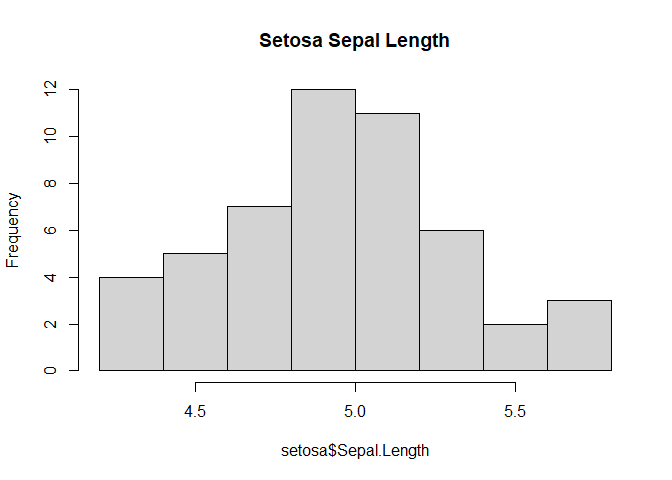
\includegraphics{Introduction_to_stats_files/figure-latex/unnamed-chunk-2-1.pdf}

\begin{Shaded}
\begin{Highlighting}[]
\NormalTok{versicolorSepLenHist \textless{}{-}}\StringTok{ }\KeywordTok{hist}\NormalTok{(versicolor}\OperatorTok{$}\NormalTok{Sepal.Length, }\DataTypeTok{main=}\StringTok{"Versicolor Sepal Length"}\NormalTok{)}
\end{Highlighting}
\end{Shaded}

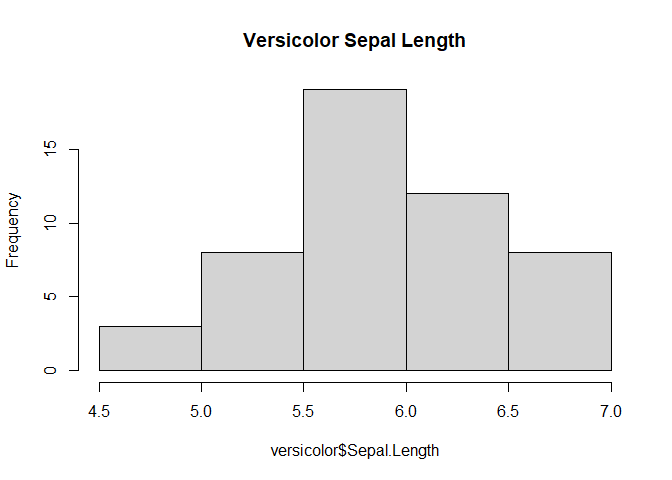
\includegraphics{Introduction_to_stats_files/figure-latex/unnamed-chunk-2-2.pdf}

\begin{Shaded}
\begin{Highlighting}[]
\NormalTok{virginicaSepLenHist \textless{}{-}}\StringTok{ }\KeywordTok{hist}\NormalTok{(virginica}\OperatorTok{$}\NormalTok{Sepal.Length, }\DataTypeTok{main=}\StringTok{"Virginica Sepal Length"}\NormalTok{)}
\end{Highlighting}
\end{Shaded}

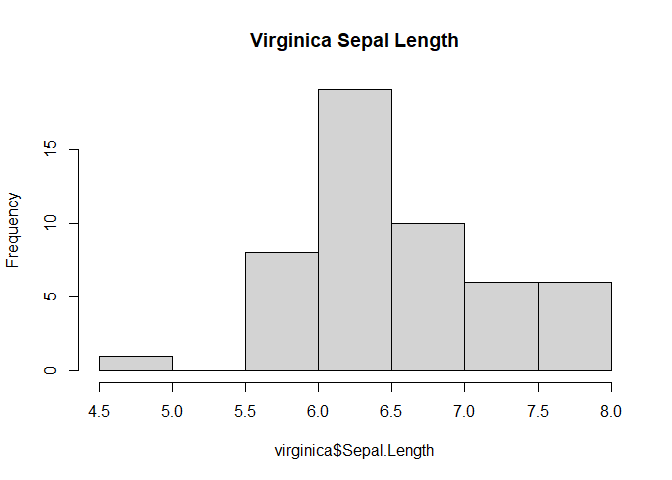
\includegraphics{Introduction_to_stats_files/figure-latex/unnamed-chunk-2-3.pdf}

\begin{Shaded}
\begin{Highlighting}[]
\NormalTok{setosaSepLenHist}
\end{Highlighting}
\end{Shaded}

\begin{verbatim}
## $breaks
## [1] 4.2 4.4 4.6 4.8 5.0 5.2 5.4 5.6 5.8
## 
## $counts
## [1]  4  5  7 12 11  6  2  3
## 
## $density
## [1] 0.4 0.5 0.7 1.2 1.1 0.6 0.2 0.3
## 
## $mids
## [1] 4.3 4.5 4.7 4.9 5.1 5.3 5.5 5.7
## 
## $xname
## [1] "setosa$Sepal.Length"
## 
## $equidist
## [1] TRUE
## 
## attr(,"class")
## [1] "histogram"
\end{verbatim}

\begin{Shaded}
\begin{Highlighting}[]
\NormalTok{versicolorSepLenHist}
\end{Highlighting}
\end{Shaded}

\begin{verbatim}
## $breaks
## [1] 4.5 5.0 5.5 6.0 6.5 7.0
## 
## $counts
## [1]  3  8 19 12  8
## 
## $density
## [1] 0.12 0.32 0.76 0.48 0.32
## 
## $mids
## [1] 4.75 5.25 5.75 6.25 6.75
## 
## $xname
## [1] "versicolor$Sepal.Length"
## 
## $equidist
## [1] TRUE
## 
## attr(,"class")
## [1] "histogram"
\end{verbatim}

\begin{Shaded}
\begin{Highlighting}[]
\NormalTok{virginicaSepLenHist}
\end{Highlighting}
\end{Shaded}

\begin{verbatim}
## $breaks
## [1] 4.5 5.0 5.5 6.0 6.5 7.0 7.5 8.0
## 
## $counts
## [1]  1  0  8 19 10  6  6
## 
## $density
## [1] 0.04 0.00 0.32 0.76 0.40 0.24 0.24
## 
## $mids
## [1] 4.75 5.25 5.75 6.25 6.75 7.25 7.75
## 
## $xname
## [1] "virginica$Sepal.Length"
## 
## $equidist
## [1] TRUE
## 
## attr(,"class")
## [1] "histogram"
\end{verbatim}

\begin{Shaded}
\begin{Highlighting}[]
\CommentTok{\#While they clearly aren\textquotesingle{}t perfectly normal, real data we look at in biology is rarely}
\CommentTok{\#exactly normal, we\textquotesingle{}ll treat this data as normal for these tests}

\CommentTok{\#We can also look at all three data sets colored differently to see if the data look}
\CommentTok{\#different next to each other, for some intuition about the results of our test}
\CommentTok{\#for that we\textquotesingle{}ll use a package called ggplot, with the original iris data frame, grouping by species}
\CommentTok{\#Also note that this isn\textquotesingle{}t a histogram, it\textquotesingle{}s something called a density plot, but for this particular exercise we can use it interchangably}

\KeywordTok{ggplot}\NormalTok{(iris, }\KeywordTok{aes}\NormalTok{(Sepal.Length, }\DataTypeTok{fill=}\NormalTok{Species)) }\OperatorTok{+}\StringTok{ }\KeywordTok{geom\_density}\NormalTok{(}\DataTypeTok{alpha=}\FloatTok{0.2}\NormalTok{)}
\end{Highlighting}
\end{Shaded}

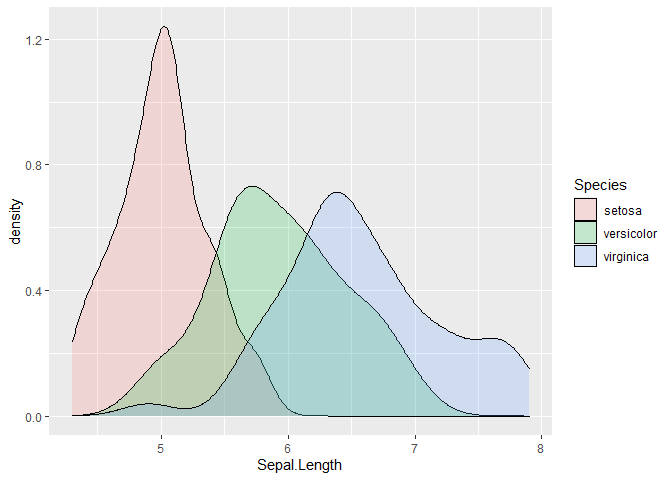
\includegraphics{Introduction_to_stats_files/figure-latex/unnamed-chunk-2-4.pdf}

So we see that our data looks (approximately) normal, and that there
appear to be differences between the data sepal length between species,
but is the differences just the effects of random sampling? Or is it
meaningful? For that we'll run our first T-test.

Every time you run a statistical test it's important to think of the
null and alternate hypotheses for the tests your running. Let's take the
test between Iris setosa and Iris virginica (setosa and verginica moving
forward).

Our null hypothesis (\(H_0\)), is that there is no difference between
sepal lengths of flowers from setosa and those from verginica. On the
other hand our alternative hypothesis (\(H_A\)), is that there IS a
difference between sepal lengths of flowers from setosa and those from
verginica. So let's run that test and spend some time with the output!

\begin{Shaded}
\begin{Highlighting}[]
\KeywordTok{t.test}\NormalTok{(setosa}\OperatorTok{$}\NormalTok{Sepal.Length, versicolor}\OperatorTok{$}\NormalTok{Sepal.Length, }\DataTypeTok{alternative =} \StringTok{"two.sided"}\NormalTok{, }\DataTypeTok{var.equal =} \OtherTok{TRUE}\NormalTok{)}
\end{Highlighting}
\end{Shaded}

\begin{verbatim}
## 
##  Two Sample t-test
## 
## data:  setosa$Sepal.Length and versicolor$Sepal.Length
## t = -10.521, df = 98, p-value < 2.2e-16
## alternative hypothesis: true difference in means is not equal to 0
## 95 percent confidence interval:
##  -1.1054165 -0.7545835
## sample estimates:
## mean of x mean of y 
##     5.006     5.936
\end{verbatim}

Before we spend any time with the code we used to run our t.test, let's
look at the output. We're going to focus on the three variables our test
output in the second row: t, df, and p-value.

\hypertarget{t}{%
\paragraph{t}\label{t}}

Starting with the t-statistic, this is the actual output of the equation
our t-test runs in the background (listed bellow). In the olden days, as
well as in previous iterations of this class, you would do this test by
hand, and then use what's called a t-table to look up the value of your
t-statistic with respect to the number of degrees of freedom (df) and
the significance value you were looking to test at. If your values
ABSOLUTE VALUE (so for our current value, about 10.5) was greater than
the one listed in the table, then your result is significant at that
level, if not you could move to a lower significance threshold and see
where your value landed. Because this is all sort of difficult to
describe, I'll link a t-table here that you can check out at your
leisure.

httpd://www.sjsu.edu/faculty/gerstman/StatPrimer/t-table.pdf

\hypertarget{df}{%
\paragraph{df}\label{df}}

Moving on to our degrees of freedom (df), this is a tougher one to
grasp, so I'll give a brief description, but I recommend that as you
move on in your statistics education you look up a few guides and
intuitive descriptions of what this means.

Generally, degrees of freedom signify how many variables that we're
looking at are free to change, given any information that's coded into
the distribution your test is using, in the case of a t-distribution the
only piece of information that comes from our data is the mean of the
distribution for each sample (don't stress to much about this point), so
for both setosa and versicolor all but one of the values could change
freely, but to keep the mean the same one value will always have to
reflect those changes to keep the mean the same. If you want to
understand this a little better, try taking 10 random values and get the
mean of those values, then replace 9 of those with a new set of random
numbers, if you also change the 10th at random, the mean is likely to
change, but if the 10th is adjusted properly, then the mean can stay the
same.

For a standard two sample t-test, the number of degrees of freedom is
the number of samples in the first group, plus the number in the second,
minus 2 (\({n_1}+{n_2}-2\)), as described above. because we have 50
samples for each species, that makes sense here!

\hypertarget{p-value}{%
\paragraph{p-value}\label{p-value}}

Our p-value is as described above, the chance that we'd get this result
by random chance, and depends on our t-statistic, along with our degrees
of freedom, our p-value is really low, meaning out t-statistic is high
given our degrees of freedom, and that our results are really likely to
represent a meaningful difference!

Now let's dive into the actual code we used to run our t-tests.

\hypertarget{one-tailed-vs-two-tailed}{%
\paragraph{One tailed vs two-tailed}\label{one-tailed-vs-two-tailed}}

You might have noticed in the line encoding this t-test,
alternative=``two.sided'', this is because the structure of our
alternative hypothesis is important for the significance of our result.
Here, our decision was to just test the idea that these species were
different, but let's say that there we were instead looking for a well
documented pattern, showing that virginica had much smaller sepals than
setosa, and rather than just looking at our data, we ran a t-test first.
The options for alternative here are ``two.sided''; meaning these are
just different, ``less''; meaning the first group is less than the
second, or ``greater'';meaning the first group has a greater mean than
the second.

\begin{Shaded}
\begin{Highlighting}[]
\KeywordTok{t.test}\NormalTok{(setosa}\OperatorTok{$}\NormalTok{Sepal.Length, versicolor}\OperatorTok{$}\NormalTok{Sepal.Length, }\DataTypeTok{alternative =} \StringTok{"greater"}\NormalTok{, }\DataTypeTok{var.equal =} \OtherTok{TRUE}\NormalTok{)}
\end{Highlighting}
\end{Shaded}

\begin{verbatim}
## 
##  Two Sample t-test
## 
## data:  setosa$Sepal.Length and versicolor$Sepal.Length
## t = -10.521, df = 98, p-value = 1
## alternative hypothesis: true difference in means is greater than 0
## 95 percent confidence interval:
##  -1.076784       Inf
## sample estimates:
## mean of x mean of y 
##     5.006     5.936
\end{verbatim}

Here we see that while our t-stat is the same, our p-value is 1, this is
because of the structure of a t-distribution, shown bellow.

\begin{Shaded}
\begin{Highlighting}[]
\KeywordTok{plot}\NormalTok{(}\ControlFlowTok{function}\NormalTok{(x) }\KeywordTok{dt}\NormalTok{(x, }\DecValTok{98}\NormalTok{), }\DecValTok{{-}11}\NormalTok{,}\DecValTok{11}\NormalTok{, }\DataTypeTok{main=}\StringTok{"t{-}distribution with 98 degrees of freedom"}\NormalTok{)}
\end{Highlighting}
\end{Shaded}

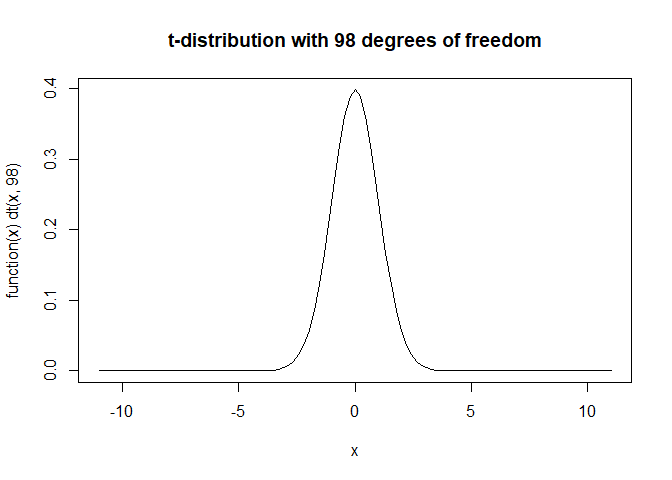
\includegraphics{Introduction_to_stats_files/figure-latex/unnamed-chunk-5-1.pdf}

With these distributions, the area under the curve (the integral for
those who are as stoked about math as they should be!) represents the
probability of all possible events (1). When we run a t-test that's two
sided, specifying just that our values are different, the actual p value
represents the area under the curve both bellow the negative value the
absolute value of our t-stat, and above the absolute value itself. If
you recall, our t-statistic is about -10.5, so if you look at this
figure you can see there's almost nothing in the described area! So our
p value is very low! This is called a two-tailed t-test, because we look
at both tails of the distribution.

Alternatively, if we specify greater as our alternative hypothesis, as
we did above, the sign of our t-statistic does matter, and we take the
value above our t-statistic. Again looking at the plot up above it's
clear that almost all of the area under the curve is above -10.5, so
there's a probability of almost 1 (100\%) that our data does NOT
meaningfully represent the pattern in our alternative hypothesis, which
makes sense looking at our data!

If we specify less, our the t-test does the opposite, which generally
would halve our p-value, but in this case our p-value is so low the
computer doesn't try to represent that number and just says it's lower
than the same REALLY low number. These are examples of one-tailed
t-tests, which just look at one tail of the distribution.

\begin{Shaded}
\begin{Highlighting}[]
\KeywordTok{t.test}\NormalTok{(setosa}\OperatorTok{$}\NormalTok{Sepal.Length, versicolor}\OperatorTok{$}\NormalTok{Sepal.Length, }\DataTypeTok{alternative =} \StringTok{"less"}\NormalTok{, }\DataTypeTok{var.equal =} \OtherTok{TRUE}\NormalTok{)}
\end{Highlighting}
\end{Shaded}

\begin{verbatim}
## 
##  Two Sample t-test
## 
## data:  setosa$Sepal.Length and versicolor$Sepal.Length
## t = -10.521, df = 98, p-value < 2.2e-16
## alternative hypothesis: true difference in means is less than 0
## 95 percent confidence interval:
##       -Inf -0.783216
## sample estimates:
## mean of x mean of y 
##     5.006     5.936
\end{verbatim}

Generally you should default to a two-tailed t-test, and only use a one
tailed when you have a REALLY strong reason to assume there's a
direction to the relationship you're looking at (ie. plants with more
light will grow larger etc.).

\hypertarget{equal-variance}{%
\paragraph{Equal variance?}\label{equal-variance}}

The other piece of the code we have here is var.equal=TRUE. This just
means we're telling the t-test to assume the variance of our two data
sets is equal. Looking at our data, this may work, but it's generally
not a safe assumption. The main reason we used it here is because if we
don't assume it, R will use a lower, more stringent number of degrees of
freedom to account for the unequal variance. We won't go into a lot of
details on this, but I'll run it bellow with that as FALSE, which is the
default, and that's the version you should use going forward.

\begin{Shaded}
\begin{Highlighting}[]
\KeywordTok{t.test}\NormalTok{(setosa}\OperatorTok{$}\NormalTok{Sepal.Length, versicolor}\OperatorTok{$}\NormalTok{Sepal.Length, }\DataTypeTok{alternative =} \StringTok{"less"}\NormalTok{, }\DataTypeTok{var.equal =} \OtherTok{FALSE}\NormalTok{)}
\end{Highlighting}
\end{Shaded}

\begin{verbatim}
## 
##  Welch Two Sample t-test
## 
## data:  setosa$Sepal.Length and versicolor$Sepal.Length
## t = -10.521, df = 86.538, p-value < 2.2e-16
## alternative hypothesis: true difference in means is less than 0
## 95 percent confidence interval:
##        -Inf -0.7830302
## sample estimates:
## mean of x mean of y 
##     5.006     5.936
\end{verbatim}

While in this case changing this option doesn't have an impact on the
outcome of our test, notice that it DOES have an impact on our degrees
of freedom, which can in many cases make a difference to our results.

That covers the basics of t-tests we'll go over here, go into the lab 1
notebook and try some for yourself!

\hypertarget{anova}{%
\subsection{ANOVA}\label{anova}}

So we've now covered how to test for a significant difference between
two groups at a time, or between one group and a theoretical
distribution, but what if we have more than two groups? While the
obvious answer might seem to be that we should just run a bunch of
t-tests and look at their flat p-values, there are actually some major
flaws with that strategy.

Think back to what a p-value is, the probability that random sampling
from whatever the hypothesized distribution of our null-hypothesis
represents can account for the patterns in our data. Now think of a data
set where our samples are grouped into 10 groups, that's 45 comparisons
(10 choose 2, \({10\choose2}\)). If we use a p-value cutoff of 0.05,
then even if all of our comparisons are significant, with a 1 in 20
chance that they're actually just different due to chance, then on
average at least 2 of those comparisons will be false positives.

There are several methods to account for this, a few of which I'll
briefly touch on at the end of this section, but the main one we're
going to focus on is called an ANOVA, or an Analysis Of Variance.

\hypertarget{whats-an-anova}{%
\subsubsection{What's an ANOVA?}\label{whats-an-anova}}

\emph{A quick note up top, anovas are another HUGE topic! There are
entire courses on how anovas work and all the variation in them, we'll
cover the basics of an archetypal anova, but if you see one that does
something different from what I'm describing, or it feels like there's
more to the story than I'm describing here, it's because these things
can get really wild really fast! Which is what makes them such a cool
tool!}

An ANOVA tests for differences between groups using groupings broken
into factors and levels, which I'll describe in just a second. The null
hypothesis of an ANOVA is that differences between groupings (and
sometimes the interaction between those groupings!) do not account for a
significant amount of the differences between individuals. That's sort
of a lot of word salad, and it's a lot easier to understand in terms of
the alternative hypothesis, which is, broadly, just that individuals
from different groups will be different.

\hypertarget{factors-and-levels}{%
\subsubsection{Factors and levels}\label{factors-and-levels}}

As I mentioned above, AMOVAs use groupings of individuals based on
\textbf{factors} and \textbf{levels}.\\
\textbf{Factors} are are ways that we can group individuals, and
\textbf{levels} are just the actual groups within those factors. So for
example, if you've got data on the fecundity (how many babies they have)
of different fish species that were all grown in different types of
habitat types, you've got two \textbf{factors}; fish species, and
habitat type, with multiple \textbf{levels} within each of those
factors. For example, within fish species you might have 5 different
species, and within habitat type you might have three different types of
rivers, all examples of levels.

\hypertarget{how-does-an-anova-work}{%
\subsubsection{How does an ANOVA work?}\label{how-does-an-anova-work}}

An ANOVA works differently from a t-test in that it's breaking down the
variation within and between groups. This can be a tough concept, so
lets run through it with our iris data, describing the conceptual steps
of an ANOVA.

First an ANOVA calculates a value called the total sum of squares
(\(SST\)). This value represents the the sum of squared deviation from
the mean (just distance from the mean) of all the values combined.

\begin{Shaded}
\begin{Highlighting}[]
\CommentTok{\#plotting our iris sepal lengh, colored by species}
\CommentTok{\#pch denotes the point shape}
\CommentTok{\#ab line adds a line where we want it, at the mean of the whole data set}
\KeywordTok{plot}\NormalTok{(iris}\OperatorTok{$}\NormalTok{Sepal.Length, }\DataTypeTok{col=}\NormalTok{iris}\OperatorTok{$}\NormalTok{Species, }\DataTypeTok{pch=}\DecValTok{20}\NormalTok{)}
\KeywordTok{abline}\NormalTok{(}\DataTypeTok{h=}\KeywordTok{mean}\NormalTok{(iris}\OperatorTok{$}\NormalTok{Sepal.Length))}
\end{Highlighting}
\end{Shaded}

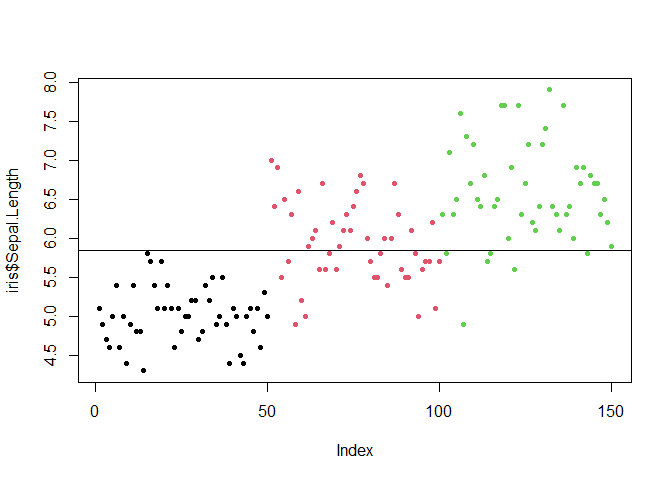
\includegraphics{Introduction_to_stats_files/figure-latex/unnamed-chunk-8-1.pdf}

Next and ANOVA calculates the error variability (\(SSE\)), the sum of
all squared deviation from the LEVEL MEAN, so the mean just within the
level of interest. So in our iris case, individuals within virginica
would be compared to the virginica mean, setosa to the setosa mean, etc
etc. here's the same plot, but with color coated means for each species!

\begin{Shaded}
\begin{Highlighting}[]
\CommentTok{\#plotting our iris sepal lengh, colored by species}
\CommentTok{\#pch denotes the point shape}
\CommentTok{\#ab line adds a line where we want it}
\KeywordTok{plot}\NormalTok{(iris}\OperatorTok{$}\NormalTok{Sepal.Length, }\DataTypeTok{col=}\NormalTok{iris}\OperatorTok{$}\NormalTok{Species, }\DataTypeTok{pch=}\DecValTok{20}\NormalTok{)}
\KeywordTok{abline}\NormalTok{(}\DataTypeTok{h=}\KeywordTok{mean}\NormalTok{(setosa}\OperatorTok{$}\NormalTok{Sepal.Length))}
\KeywordTok{abline}\NormalTok{(}\DataTypeTok{h=}\KeywordTok{mean}\NormalTok{(versicolor}\OperatorTok{$}\NormalTok{Sepal.Length), }\DataTypeTok{col=}\StringTok{"red"}\NormalTok{)}
\KeywordTok{abline}\NormalTok{(}\DataTypeTok{h=}\KeywordTok{mean}\NormalTok{(virginica}\OperatorTok{$}\NormalTok{Sepal.Length), }\DataTypeTok{col=}\StringTok{"green"}\NormalTok{)}
\end{Highlighting}
\end{Shaded}

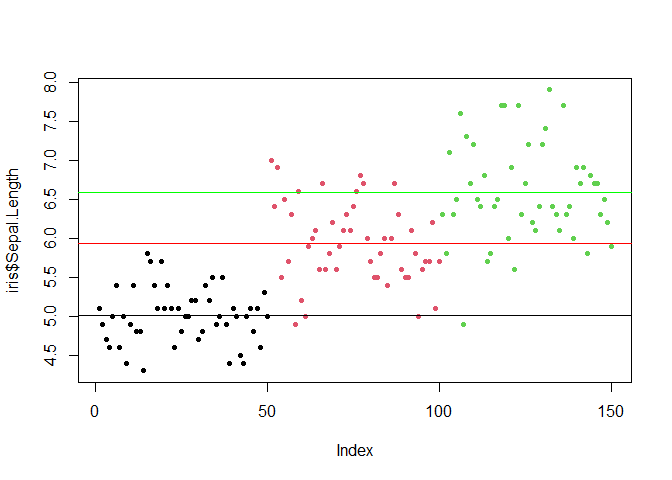
\includegraphics{Introduction_to_stats_files/figure-latex/unnamed-chunk-9-1.pdf}

Note that \(SST\) will always be greater than or equal to \(SSE\), with
the remaining variance being from within the factor itself (\(SSF\)),
and so \[SST=SSE+SSF\].

That's not an equation you necessarily have to know, but just understand
that an ANOVA uses this to break down the variation that each level
accounts for, to understand whether the differences between those levels
is meaningful.

The way this works is by delving the sum of squares at a given level
(\(SSE/T/F\)) by the degrees of freedom for that sum of squares, to the
compute what's called the mean square variability (\(MS\)). Then it
devides the \(MS\) for the given factor, by the \(MS\) for our error
term to get a statistic called F that you then compare to table similar
to the one described above. This is all fairly complicated to see
written out, so lets run an example on our iris data.

\begin{Shaded}
\begin{Highlighting}[]
\CommentTok{\#first we run our anova using the aov function}
\CommentTok{\#we specify the formula for our ANOVA using the syntax (dependent.variable \textasciitilde{} explanaotry.variable(s))}
\CommentTok{\#We use the summary function because, as you can see, the aov output itself doesn\textquotesingle{}t give us a p value (Pr(\textgreater{}F) in the summary)}

\NormalTok{iris.aov \textless{}{-}}\StringTok{ }\KeywordTok{aov}\NormalTok{(Sepal.Length}\OperatorTok{\textasciitilde{}}\NormalTok{Species, }\DataTypeTok{data=}\NormalTok{iris)}
\KeywordTok{print}\NormalTok{(}\StringTok{"*******aov function output **********"}\NormalTok{)}
\end{Highlighting}
\end{Shaded}

\begin{verbatim}
## [1] "*******aov function output **********"
\end{verbatim}

\begin{Shaded}
\begin{Highlighting}[]
\NormalTok{iris.aov}
\end{Highlighting}
\end{Shaded}

\begin{verbatim}
## Call:
##    aov(formula = Sepal.Length ~ Species, data = iris)
## 
## Terms:
##                  Species Residuals
## Sum of Squares  63.21213  38.95620
## Deg. of Freedom        2       147
## 
## Residual standard error: 0.5147894
## Estimated effects may be unbalanced
\end{verbatim}

\begin{Shaded}
\begin{Highlighting}[]
\KeywordTok{print}\NormalTok{(}\StringTok{"******* summary output ****"}\NormalTok{)}
\end{Highlighting}
\end{Shaded}

\begin{verbatim}
## [1] "******* summary output ****"
\end{verbatim}

\begin{Shaded}
\begin{Highlighting}[]
\KeywordTok{summary}\NormalTok{(iris.aov)}
\end{Highlighting}
\end{Shaded}

\begin{verbatim}
##              Df Sum Sq Mean Sq F value Pr(>F)    
## Species       2  63.21  31.606   119.3 <2e-16 ***
## Residuals   147  38.96   0.265                   
## ---
## Signif. codes:  0 '***' 0.001 '**' 0.01 '*' 0.05 '.' 0.1 ' ' 1
\end{verbatim}

The summary output above gives us everything we need to understand the
ANOVA. We can see for our species level the sum of squares, the \(MS\)
value, the and the degrees of freedom, similarly we see it for our error
term (Residuals), along with our F and p values! To make sure you
understand how to get to that F statistic from our sum of squares and
degrees of freedom, work through it with a pen and paper! (this will be
in the lab for this section!)

\hypertarget{a-few-more-a-note-vas-notes-on-anovas-im-kind-of-a-fun-ta}{%
\subsubsection{A few more A-Note-VAs (notes on ANOVAs, I'm kind of a fun
TA?)}\label{a-few-more-a-note-vas-notes-on-anovas-im-kind-of-a-fun-ta}}

So what we've just done is basically the simplest version of an ANOVA,
but note that we can also have multiple explanatory variables (factors),
which can interact, or be nested within one-another.

Interacting terms basically just mean you've got two factors that
interact (pretty straight forward right??). Think wayyy back to the top
of this section where I talked about fish species and habitats. It's
entirely possible that a given habitat will have a different impact on
fish of different species, so not only could fish and species explain
some of the variation, fish species combined with a given habitat can
have an impact. The way we denote that in an r formula would be
(fecundity \textasciitilde{} species + habitat + species*habitat),
because we want to look at the effect of species, plus the effect of
habitat, plus the effect of species combined with the habitat it's in.

Another thing to be aware of is a relationship called nesting. Nesting
just means that one factor subdivides another factor, so it should be
considered with subsets of another factor. For example, lets say that
for each of the fish species we were considering, we have three
genotype. If for example we have 4 fish species, if we just include
genotype as its own fully independent factor, then we're dividing out
data up into 12 levels that are really not independent of our species
variable. Instead we would say that genotype is a nested variable within
species. That's designated in R as follows (fecundity \textasciitilde{}
species/genotype), and will better split up variance with genotype
within habitat.

These relationships can get complex as you design experiments, so think
about them as you move on with your scientific careers! Not accounting
for an interaction or a nesting relationship can be the difference
between a meaningful result and junk science! Also I still get tripped
up on this stuff, as does every other person I know who uses these so
don't be afraid to ask for help!

\hypertarget{other-ways-to-account-for-multiple-groups}{%
\subsubsection{Other ways to account for multiple
groups}\label{other-ways-to-account-for-multiple-groups}}

As promised here are a couple of other ways to work with multiple groups
your testing between. I won't go into detail on either, so do some super
fun googling if you're interested! Highly recommended!

First you can run a t-test with a lower significance cutoff, there are
several methods for this, and they're often referred to as
\textbf{multiple hypothesis corrections}. This lessens the chance that
you're calling a non significant difference significant.

The other methods I'll mention is something called a Tukey test. A Tuky
test works very similar to running a t-test on all comparisons, and will
give a pairwise, corrected p-value, for all comparisons.

The draw to both of these methods is that they give you specific p
values for comparisons, while an ANOVA will just tell you that the
grouping makes a difference. I would recommend always running an ANOVA
first though, because otherwise you'll be searching through a massive
list of p-values when it's possible none are significant in the first
place. An ANOVA can save you that trouble!

Now head back to the lab 1 notebook and do the ANOVA section of the lab!

\hypertarget{chi-squared}{%
\subsection{Chi-Squared}\label{chi-squared}}

Next we'll cover a chi-squared (\(\chi^2\)) test. We're going to go a
bit less in depth here having covered the t-test and AMOVAs in a lot of
detail, but generally the way the test works is the same, although the
test itself is very different. You get a test statistic based on your
data which is then compared to a chi-squared distribution via a values
table to understand how the data stacks up against your hypotheses.

A chi-squared test is used to tell whether a set of count data differs
from a null expectation, which will generally just that all groups have
a proportional number of individuals (this will be clearer in a second).
The number of degrees of freedom for a chi-squared test is either the
number of columns in your contingency table minus 1 (\(c-1\)), or the
following, where r represents rows, and c represents columns:
\[df=(r-1)(c-1)\]

Furthermore, the function for the chi squared statistic is
\[\sum{\frac{(observed-expected)^2}{expected}}\]\\
over all values in your contingency table.

To understand how we get our expected values, lets look at some data
from an R package called MASS on a survey testing if peoples smoking
habits (rows), were related to their exercise habits.

\begin{Shaded}
\begin{Highlighting}[]
\CommentTok{\#load the package}
\KeywordTok{library}\NormalTok{(MASS)}
\NormalTok{data \textless{}{-}}\StringTok{ }\KeywordTok{table}\NormalTok{(survey}\OperatorTok{$}\NormalTok{Smoke, survey}\OperatorTok{$}\NormalTok{Exer)}
\NormalTok{data}
\end{Highlighting}
\end{Shaded}

\begin{verbatim}
##        
##         Freq None Some
##   Heavy    7    1    3
##   Never   87   18   84
##   Occas   12    3    4
##   Regul    9    1    7
\end{verbatim}

This type of data table that has various groups along with the count of
individuals in those groups is called a contingency table.

So here we see our observed values, but how do we get our expected
values? To do that we need the total number of individuals, along with
the proportion of those individuals in each row and column.

\begin{Shaded}
\begin{Highlighting}[]
\NormalTok{total \textless{}{-}}\StringTok{ }\KeywordTok{sum}\NormalTok{(data)}
\NormalTok{total}
\end{Highlighting}
\end{Shaded}

\begin{verbatim}
## [1] 236
\end{verbatim}

\begin{Shaded}
\begin{Highlighting}[]
\KeywordTok{rowSums}\NormalTok{(data)}\OperatorTok{/}\NormalTok{total}
\end{Highlighting}
\end{Shaded}

\begin{verbatim}
##      Heavy      Never      Occas      Regul 
## 0.04661017 0.80084746 0.08050847 0.07203390
\end{verbatim}

\begin{Shaded}
\begin{Highlighting}[]
\KeywordTok{colSums}\NormalTok{(data)}\OperatorTok{/}\NormalTok{total}
\end{Highlighting}
\end{Shaded}

\begin{verbatim}
##       Freq       None       Some 
## 0.48728814 0.09745763 0.41525424
\end{verbatim}

So above we have the proportions for each row (the fraction of the total
that row accounts for, the (number of individuals in that row)/(total
number of individuals)), and the same for each column. To get our
expected proportion we just multiply these values for a given cell, and
then multiply the value by the total number of individuals.

Bellow is an example value for heavy smokers who exercise frequently.

\begin{Shaded}
\begin{Highlighting}[]
\NormalTok{expectedHeavyFreq \textless{}{-}}\StringTok{ }\DecValTok{236}\OperatorTok{*}\FloatTok{0.0466}\OperatorTok{*}\FloatTok{0.487}
\NormalTok{expectedHeavyFreq}
\end{Highlighting}
\end{Shaded}

\begin{verbatim}
## [1] 5.355831
\end{verbatim}

Let's also get a value for our degrees of freedom, just for practice.
Remember we have 4 rows, and 3 columns.

\begin{Shaded}
\begin{Highlighting}[]
\NormalTok{r \textless{}{-}}\StringTok{ }\DecValTok{4}
\NormalTok{c \textless{}{-}}\StringTok{ }\DecValTok{3}
\NormalTok{df \textless{}{-}}\StringTok{ }\NormalTok{(r}\DecValTok{{-}1}\NormalTok{)}\OperatorTok{*}\NormalTok{(c}\DecValTok{{-}1}\NormalTok{)}
\NormalTok{df}
\end{Highlighting}
\end{Shaded}

\begin{verbatim}
## [1] 6
\end{verbatim}

Let's now go ahead and run a chi squared test in R and see if our data
differ from our null expectation!

\begin{Shaded}
\begin{Highlighting}[]
\KeywordTok{chisq.test}\NormalTok{(data)}
\end{Highlighting}
\end{Shaded}

\begin{verbatim}
## Warning in chisq.test(data): Chi-squared approximation may be incorrect
\end{verbatim}

\begin{verbatim}
## 
##  Pearson's Chi-squared test
## 
## data:  data
## X-squared = 5.4885, df = 6, p-value = 0.4828
\end{verbatim}

So our p-value is 0.4828, but what does that mean? It's easy to just say
``that our data is not significantly different from our null
expectation!'' But we're scientists not statisticians! I'll sometimes
ask you to you to interpret a test, and unless I'm really specific I'm
always asking for a real, biological interpenetration, you've been
warned!

So here we can't reject our null hypothesis. Think about what that
means, the number of individuals for every group (for example occasional
smokers who exercise sometimes) is about what it would be if you just
took the proportion of people who smoke occasionally and multiplied it
by the proportion of people who exercise sometimes. Generally speaking,
it means that these two groupings don't seem to have a meaningful effect
on each other, so how much someone exercises doesn't seem to have an
impact on how much they smoke, or vica-verca.

Now take what you know about chi-squared tests and do the corresponding
section of lab 1!

\hypertarget{correlation}{%
\subsection{Correlation}\label{correlation}}

I'm going to assume most of you have heard of correlation's before, so I
won't spend a lot of time motivating this one. Generally a correlation
measures the strength of the relationship between two variables, ie,
when X gets larger does Y consistently get larger? Smaller? We measure
the strength of that relationship using correlation coefficient, for
this we'll focus on one specifically called \textbf{Pearson's
correlation coefficient}, but you should know that there are other
methods out there! We almost always represent correlation coefficients
with the term \textbf{r} (note that it's lower case!).

We calculate r as follows:
\[r=\frac{\sum{xy}}{\sqrt{\sum{x^2}\sum{y^2}}}\]

Where an r of 1 means there's a perfect positive correlation (when x
increases, y ALWAYS increases by an amount that is exactly
proportional), and r of 0 means there's no correlation, and an r of -1
means that there's a perfect negative correlation.

\hypertarget{its-cool-to-be-cautious-when-calculating-correlations}{%
\subsubsection{it's Cool to be Cautious when Calculating
Correlations}\label{its-cool-to-be-cautious-when-calculating-correlations}}

There are a few things to be careful of when you're calculating and
using correlations! First off remember, a correlation DOES NOT IMPLY
CAUSATION! This just means that just because two things have a high r
value, does not mean that one causes the other! A classic example is
that drownings are tightly correlated with ice cream consumption per
capita every year, but only because more people are around water and
eating ice cream during the summer! There are some great sights for
this, for example the web site
\url{https://www.tylervigen.com/spurious-correlations} points out that
there's an omminous r of 0.666 between drownings by falling into a pool
in a year with the number of films Nick Cage has appeared in that year.
It's possible that it's all because of people staring at TVs, distracted
while walking next to their pool thinking ``is that Nick Cage?'', but
it's more likely what's called a spurious correlation, meaning there's
no real relationship between the two variables. Make sure that you never
assume causation for a correlation, and make sure the ones you believe
make some sense!

Another factor to be cautious of when calculating correlations is that
all correlations with the methods we're using are linear correlations.
While this does not sound super important, you might be fitting a
relationship that doesn't make sense to your data, and drawing the wrong
conclusions from it! Always look at your data! Plot it! Stare at it!

Finally, related to the above point, a correlation driven by an outline
is quantitatively the same as a correlation driven by a real
relationship, always look for outline (points way outside the rest of
your data, or points that just don't make any sense) before you run a
correlation. Just to reiterate - Always look at your data! Plot it!
Stare at it!

Now let's get back to that sweet sweet iris data! Let's look for a
correlation between sepal length and sepal width. It seems, without
taking a look, like longer petals could be wider, as they might just be
larger overall, but let's take a closer look!

\begin{Shaded}
\begin{Highlighting}[]
\CommentTok{\#first let\textquotesingle{}s look at our data on a plot}
\KeywordTok{plot}\NormalTok{(iris}\OperatorTok{$}\NormalTok{Sepal.Length, iris}\OperatorTok{$}\NormalTok{Sepal.Width)}
\end{Highlighting}
\end{Shaded}

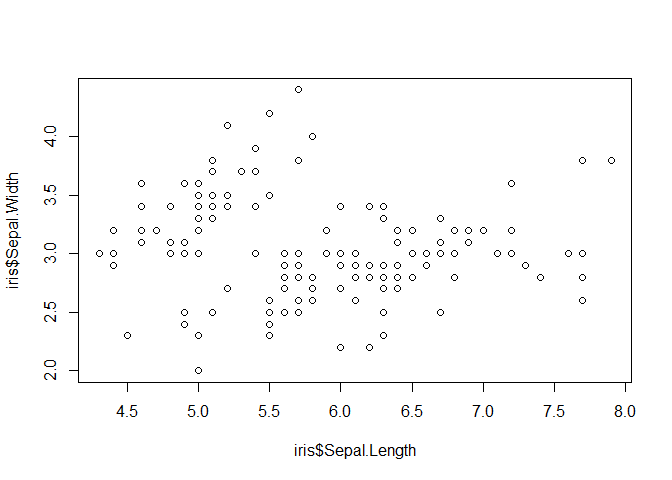
\includegraphics{Introduction_to_stats_files/figure-latex/unnamed-chunk-16-1.pdf}

First it's important to note that we don't see any obvious outlines or
clear non-linear relationships. Then it's interesting to note, there
isn't an obvious, strong relationship, so if we do get a high r value we
know something is up we're not seeing.

Also note, we can run a simple correlation to just get an r value, or we
can run a correlation test, which will also list off degrees of freedom
and a significance value. Both the r and the significance value are
useful so I would recommend using the ``cor.test'' function over the
simple cor function.

\begin{Shaded}
\begin{Highlighting}[]
\CommentTok{\#now let\textquotesingle{}s run our actual correlation test}
\KeywordTok{cor}\NormalTok{(iris}\OperatorTok{$}\NormalTok{Sepal.Length, iris}\OperatorTok{$}\NormalTok{Sepal.Width)}
\end{Highlighting}
\end{Shaded}

\begin{verbatim}
## [1] -0.1175698
\end{verbatim}

\begin{Shaded}
\begin{Highlighting}[]
\KeywordTok{cor.test}\NormalTok{(iris}\OperatorTok{$}\NormalTok{Sepal.Length, iris}\OperatorTok{$}\NormalTok{Sepal.Width)}
\end{Highlighting}
\end{Shaded}

\begin{verbatim}
## 
##  Pearson's product-moment correlation
## 
## data:  iris$Sepal.Length and iris$Sepal.Width
## t = -1.4403, df = 148, p-value = 0.1519
## alternative hypothesis: true correlation is not equal to 0
## 95 percent confidence interval:
##  -0.27269325  0.04351158
## sample estimates:
##        cor 
## -0.1175698
\end{verbatim}

We see that not only was there not a strong, significant positive
relationship between sepal length and width, there was even a
(non-significant) slight negative relationship! So we see here that
sepals on our iris species can be long, or wide, or both, not just
larger or smaller! Aren't stat's awesome??

As usual, move back to the lab 1 notebook and come back when you've
worked through correlations!

\hypertarget{regression}{%
\subsection{Regression}\label{regression}}

Regressions are really similar to correlations, but with one important
difference, a regression does imply a causative relationship, because we
are actively fitting our dependent variable as a function of our
independent variable. This is super helpful when you have a clear
relationship in mind, but note you're still driving, if you put in a
relationship that doesn't actually make any sense, but a regression
fits, you'll get a meaningless significant result!

For this lab we're going to focus on linear regressions, but note that
just about any relationship you can have between two mathematical
variables you can fit as a regression (exponential, logistic,
logarithmic, trigonometric, etc.), like ANOVAs there are entire courses
on regression, so there's lots you can dive into if you get excited
about them!

The form of linear regression is as follows: \[Y = a + bX + \epsilon\]\\
where Y is our dependent variable, a and b are our regression
coefficients (what we're looking to find), X is our independent
variable, and \(\epsilon\) is our residual error, or just anything not
accounted for by our regression coefficients.

We won't get into the details of how the computer actually calculates a
and b, but if you're interested it's generally in the field of machine
learning, often with a technique called gradient decent. All you need to
know is that the computer finds an a and b the minimizes the squared
distance of data points from the regression line.

With regressions we use a value called \(R^2\) to understand how good
the fit of our relationship to our data is, which is called the
coefficient of variation. \(R^2\) represents the proportion of variation
in Y explained by the regression, so it varies from 0 to 1.

Note that in a simple linear regression \(R^2\) is the same as the
Pearson correlation coefficient (r) squared, but that this is a special
case and you should always make sure that you're using the appropriate
test, and the appropriate terms. This will make life much easier when
some day you need to model more complex relationships!

It's also useful to note the null and alternative hypotheses of a
regression. \(H_0\) just states that b=0 (the line is flat, there is no
meaningful relationship), whereas \(H_A\) is that the line is not flat,
b does not equal 0.

Finally, before we get into our last (!!!) statistical example for this
lab, a word of warning. A regression will give you an equation that you
could, in theory use with whatever values you want, which seems really
useful! But always be cautious using that relationship to make estimates
outside the range of the data you collected. The relationship may be
different for values much larger or smaller than yours, so always be
careful making big assumptions!

Now lets dive into a data set built into R that should be good for this
course! We'll look at the ``trees'' data set, which gives data on the
dimensions of 31 felled black cherry trees. Let's say our alternative
hypothesis is that taller trees have a larger volume, with the null
hypothesis being that height has no effect on volume.

\begin{Shaded}
\begin{Highlighting}[]
\CommentTok{\#First lets read in, and look at our data to make sure we don\textquotesingle{}t have any crazy outliers, or obvious non{-}linear relationships}
\KeywordTok{data}\NormalTok{(trees)}
\KeywordTok{plot}\NormalTok{(trees}\OperatorTok{$}\NormalTok{Height, trees}\OperatorTok{$}\NormalTok{Volume)}
\end{Highlighting}
\end{Shaded}

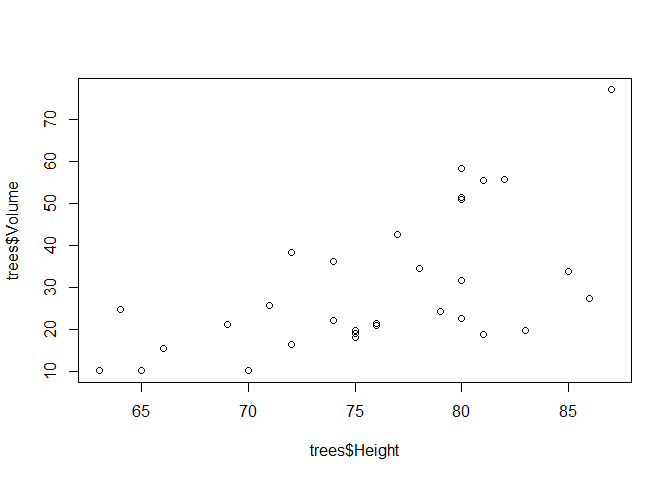
\includegraphics{Introduction_to_stats_files/figure-latex/unnamed-chunk-18-1.pdf}
So we see above that there are no obvious outlines or clear non-linear
relationships, so lets go ahead a fit a simple regression to our data.

To fit a regression to data in r we actually fit something called a
linear model with the function lm. Like with our ANOVA, we need to
assign our model to a variable to then summarize it.

\begin{Shaded}
\begin{Highlighting}[]
\NormalTok{model \textless{}{-}}\StringTok{ }\KeywordTok{lm}\NormalTok{(}\DataTypeTok{formula =}\NormalTok{ Volume }\OperatorTok{\textasciitilde{}}\StringTok{ }\NormalTok{Height, }\DataTypeTok{data=}\NormalTok{trees)}
\KeywordTok{summary}\NormalTok{(model)}
\end{Highlighting}
\end{Shaded}

\begin{verbatim}
## 
## Call:
## lm(formula = Volume ~ Height, data = trees)
## 
## Residuals:
##     Min      1Q  Median      3Q     Max 
## -21.274  -9.894  -2.894  12.068  29.852 
## 
## Coefficients:
##             Estimate Std. Error t value Pr(>|t|)    
## (Intercept) -87.1236    29.2731  -2.976 0.005835 ** 
## Height        1.5433     0.3839   4.021 0.000378 ***
## ---
## Signif. codes:  0 '***' 0.001 '**' 0.01 '*' 0.05 '.' 0.1 ' ' 1
## 
## Residual standard error: 13.4 on 29 degrees of freedom
## Multiple R-squared:  0.3579, Adjusted R-squared:  0.3358 
## F-statistic: 16.16 on 1 and 29 DF,  p-value: 0.0003784
\end{verbatim}

Again here we get a lot of information, but what's really important for
our purposes is in the last two rows, our R\^{}2 value and significance.
We see that we have an R\^{}2 above 0, and a p value bellow 0.05, so
there is in fact a significant relationship between height and volume!
Which makes sense! Go team!

I hope this has all be informative, and will be going forward as we work
with data throughout this course! If you have any questions let me
(Alex) know so I can clarify them!

Now go ahead back to the lab 1 file and finish up with the regression
section! See you all next week!

\end{document}
